\documentclass[11pt, aspectratio=169]{beamer}

\usepackage[utf8]{inputenc}
\usepackage{tikz}
\usepackage[english]{babel}
\usepackage{svg}
\usepackage{eurosym}
\usepackage{subfig}
\usepackage{pgfgantt}
\usepackage[export]{adjustbox}

% \usepackage[table]{xcolor}

\usepackage{color, colortbl}
\definecolor{Gray}{rgb}{0.8,.8,.8}

\usepackage{soul}
\usepackage{eurosym}

%\usepackage[shortlabels]{enumitem}
\usepackage[font=scriptsize,justification=centering]{caption}
\usepackage{movie15}
\usepackage{tikz}
\usetikzlibrary{arrows,shapes,positioning,shadows,trees}
\graphicspath{{figures/}}

%----------------------------------------------------------------------------------------
%   TITLE PAGE INFORMATION.
%----------------------------------------------------------------------------------------
\author{S. Björk, J. Hooper, J. M. Inga, H. Magnusson, A. Śmiałek}
\title{InfraRed Imaging of astronomical targets with a Stabilised Camera}
\subtitle{IRISC}
\institute{ESA ESTEC, Noordwijk}
\date{17 May 2019}
%\subject{} 

%----------------------------------------------------------------------------------------
%   SETUP LAYOUT.
%----------------------------------------------------------------------------------------
\usepackage{theme/beamerthemeWarsawLTU}
%\usetheme{Warsaw}


\begin{document}
%----------------------------------------------------------------------------------------
%   TITLE PAGE.
%----------------------------------------------------------------------------------------

{\setbeamertemplate{logo}{}
\begin{frame}
\titlepage
\begin{tikzpicture}[remember picture,overlay]
    \node[xshift=13cm,yshift=-1.025\textheight,anchor=north west] at (current page.north west){%
    
\includegraphics[width=2cm]{theme/LTU_logo.jpg}};
\end{tikzpicture}
\end{frame}
}

%----------------------------------------------------------------------------------------
%   TABLE OF CONTENTS.
%----------------------------------------------------------------------------------------
\begin{frame}[t]{Table of Contents}
\vspace{-0.3cm}
    \begin{columns}[t]
        \begin{column}{.5\textwidth}
            \tableofcontents[sections={1-2}]
        \end{column}
        \begin{column}{.5\textwidth}
            \tableofcontents[sections={3-5}]
            \vspace{-.2cm}
            \tableofcontents[sections=6,hidesubsections]
        \end{column}
    \end{columns}
\end{frame}

%----------------------------------------------------------------------------------------
%   INTRODUCTION / EXPERIMENT OVERVIEW.
%----------------------------------------------------------------------------------------
\section{Experiment Overview}
\begin{frame}[c]{Experiment Overview}
    \begin{columns}[t]
        \begin{column}{.4\textwidth}
            \centering
            \vspace{2cm}\\
            \large{InfraRed Imaging of astronomical targets with a Stabilised Camera}
        \end{column}
        \begin{column}{.6\textwidth}
        \vspace{-.5cm}
            \begin{figure}
                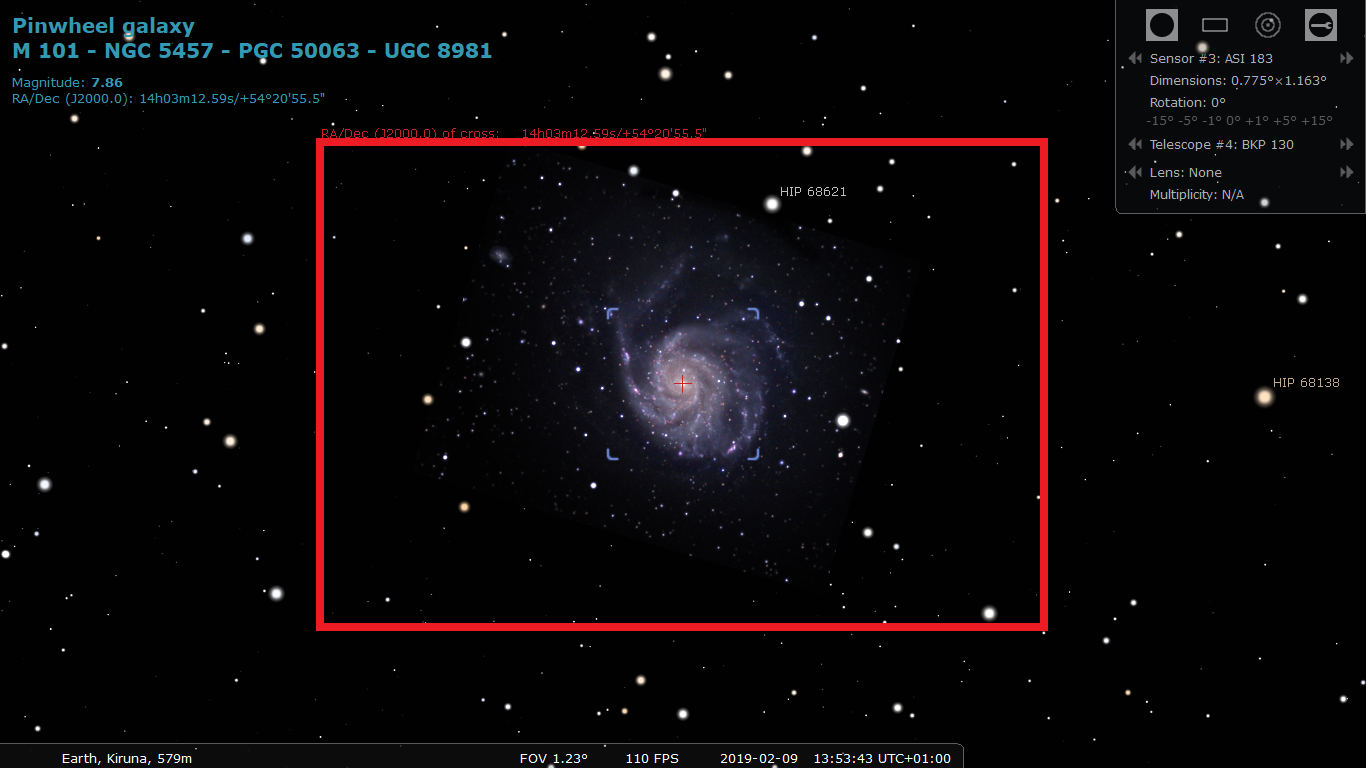
\includegraphics[height=.45\textheight]{overview/Pinwheel_BKP130.png}
                %%%% TODO: newer CAD model
                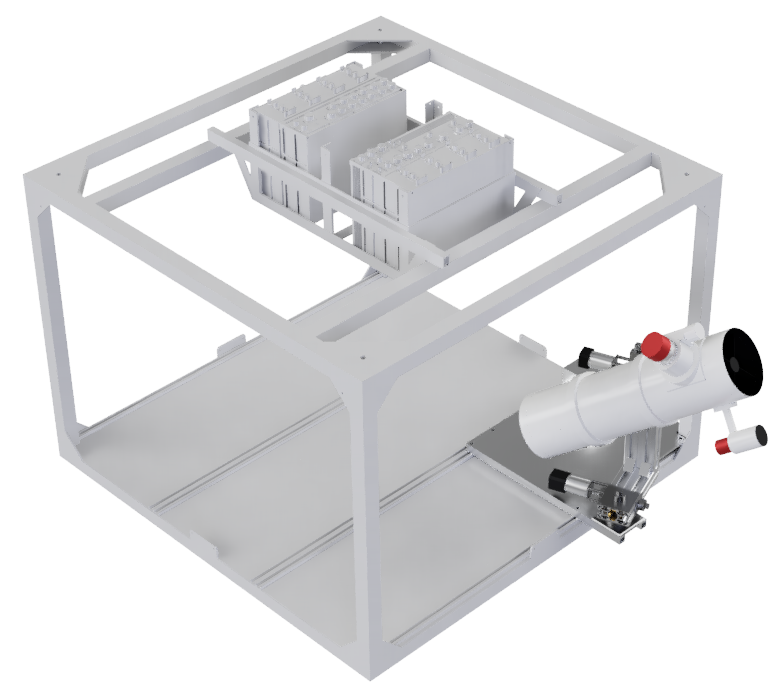
\includegraphics[height=.5\textheight]{overview/experiment_overview.png}
            \end{figure}
        \end{column}
    \end{columns}
\end{frame}


%----------------------------------------------------------------------------------------
%   SYSTEM.
%----------------------------------------------------------------------------------------
\section{System}
%   CONSTRUCTION. -----------------------------------------------------------------------
\subsection{Construction}
%   THERMAL. ----------------------------------------------------------------------------

\subsection{Thermal}
\begin{frame}[c]{Thermal}
    \begin{figure}
        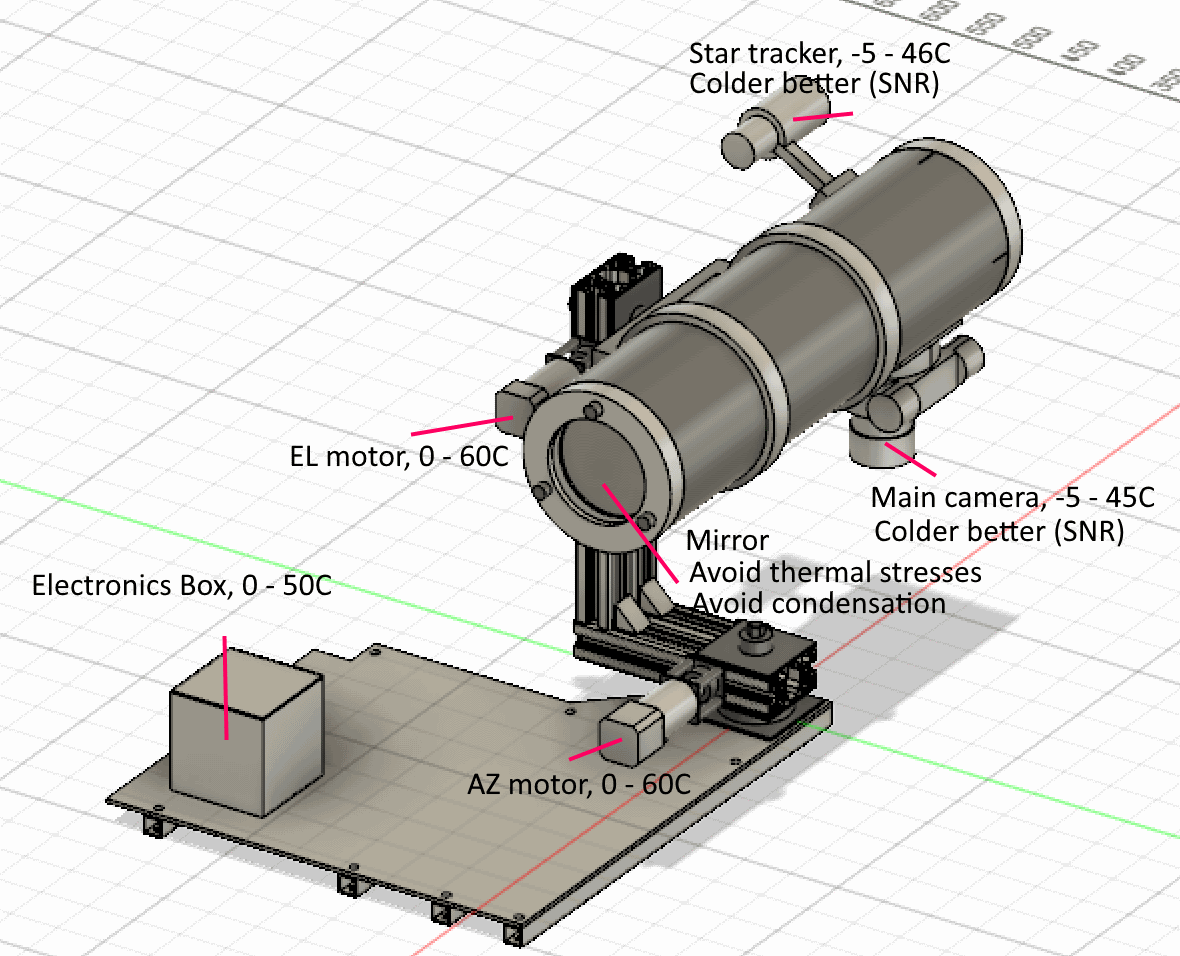
\includegraphics[height=1\textheight]{images/thermalsystem.png}
    \end{figure}
\end{frame}

\begin{frame}[c]{Thermal}
    \begin{figure}[h!]
        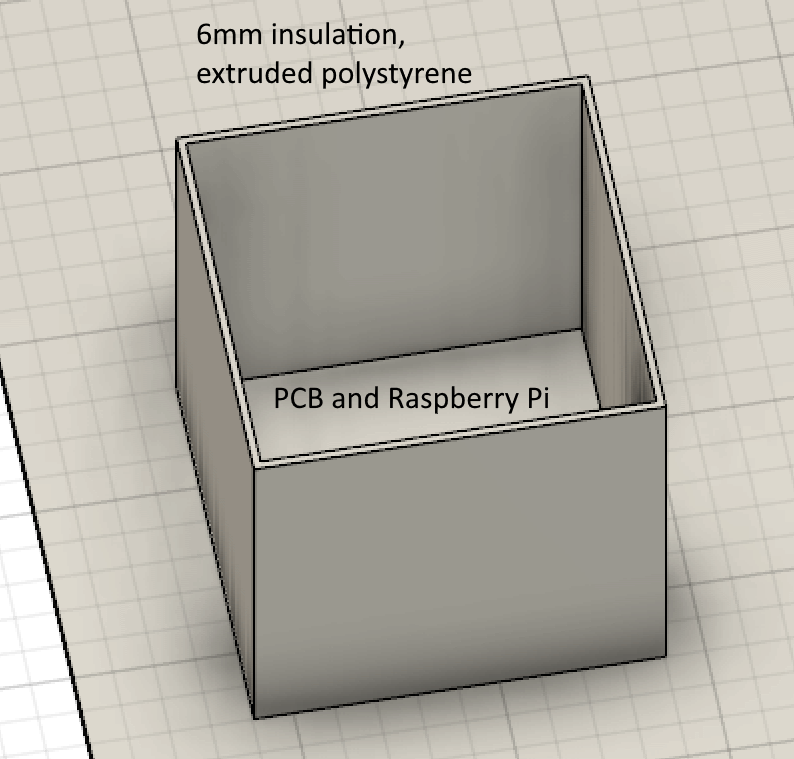
\includegraphics[height=.7\textheight]{images/box.png}
        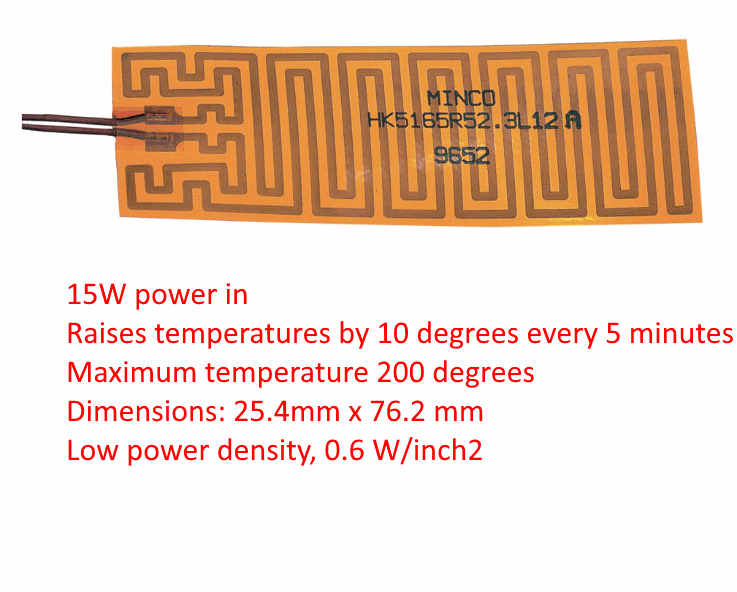
\includegraphics[height=.7\textheight]{images/mincoheatingpad.png}
    \end{figure}
\end{frame}

\begin{frame}[c]{Thermal}
    \begin{figure}[h!]
        \centering
        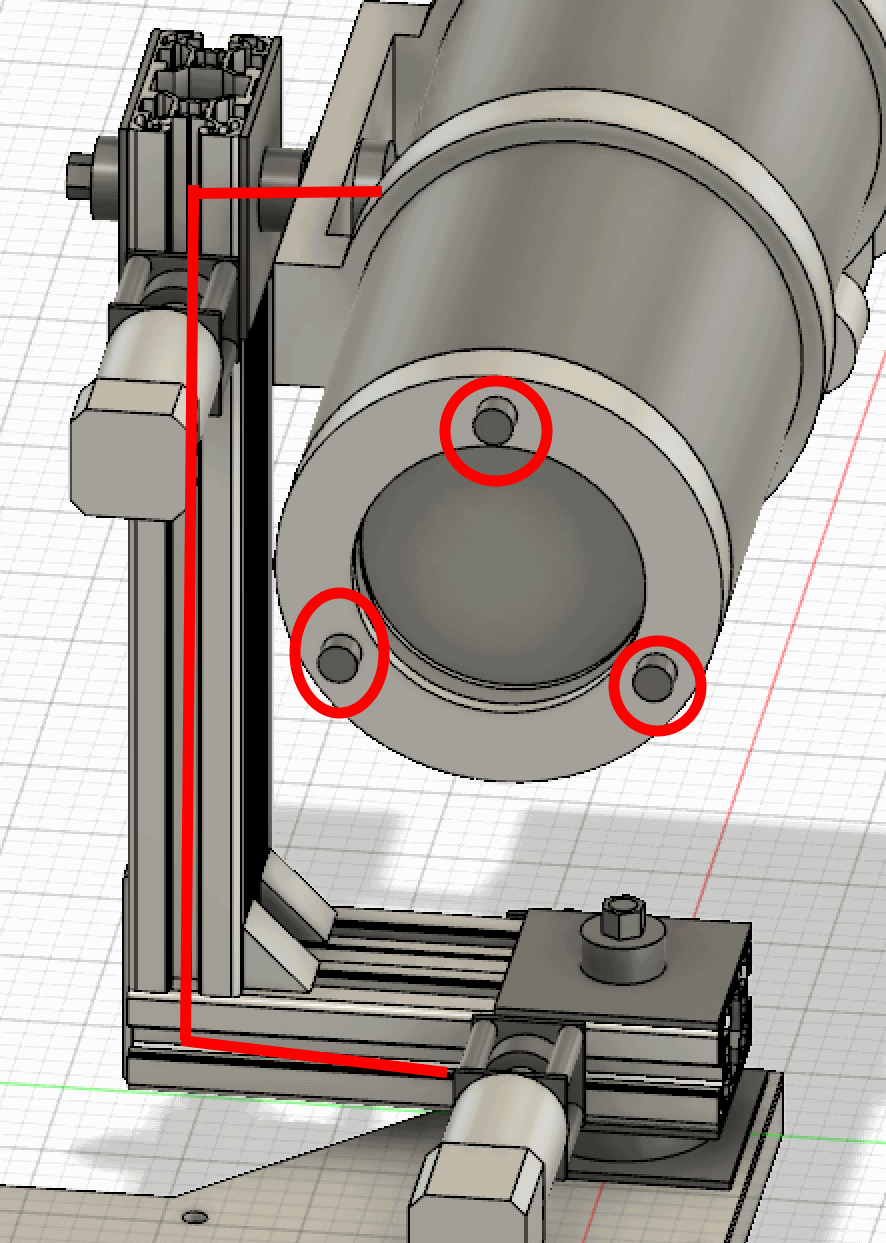
\includegraphics[height=.7\textheight]{images/thermalpaths.png}
        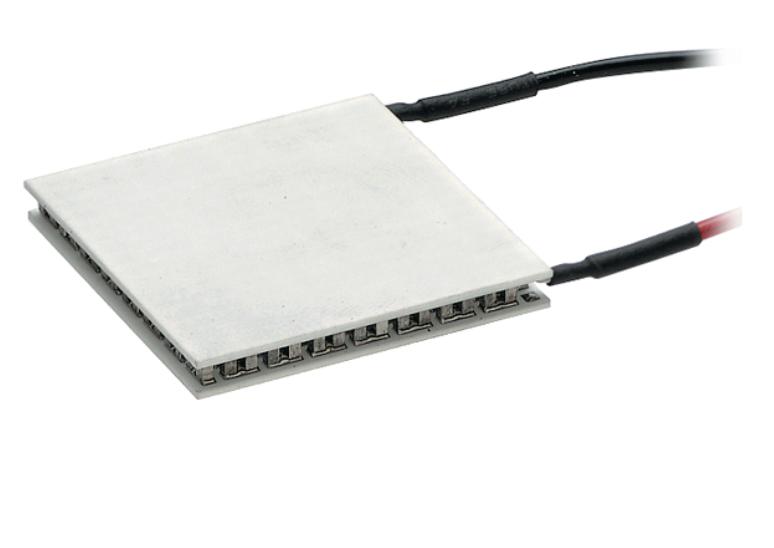
\includegraphics[height=.7\textheight]{images/peltierelement.png}
    \end{figure}
\end{frame}

%   ELECTRICAL. -------------------------------------------------------------------------
\subsection{Electrical Setup}
    \begin{frame}[c]{Electrical - Setup}
   		\begin{figure}
            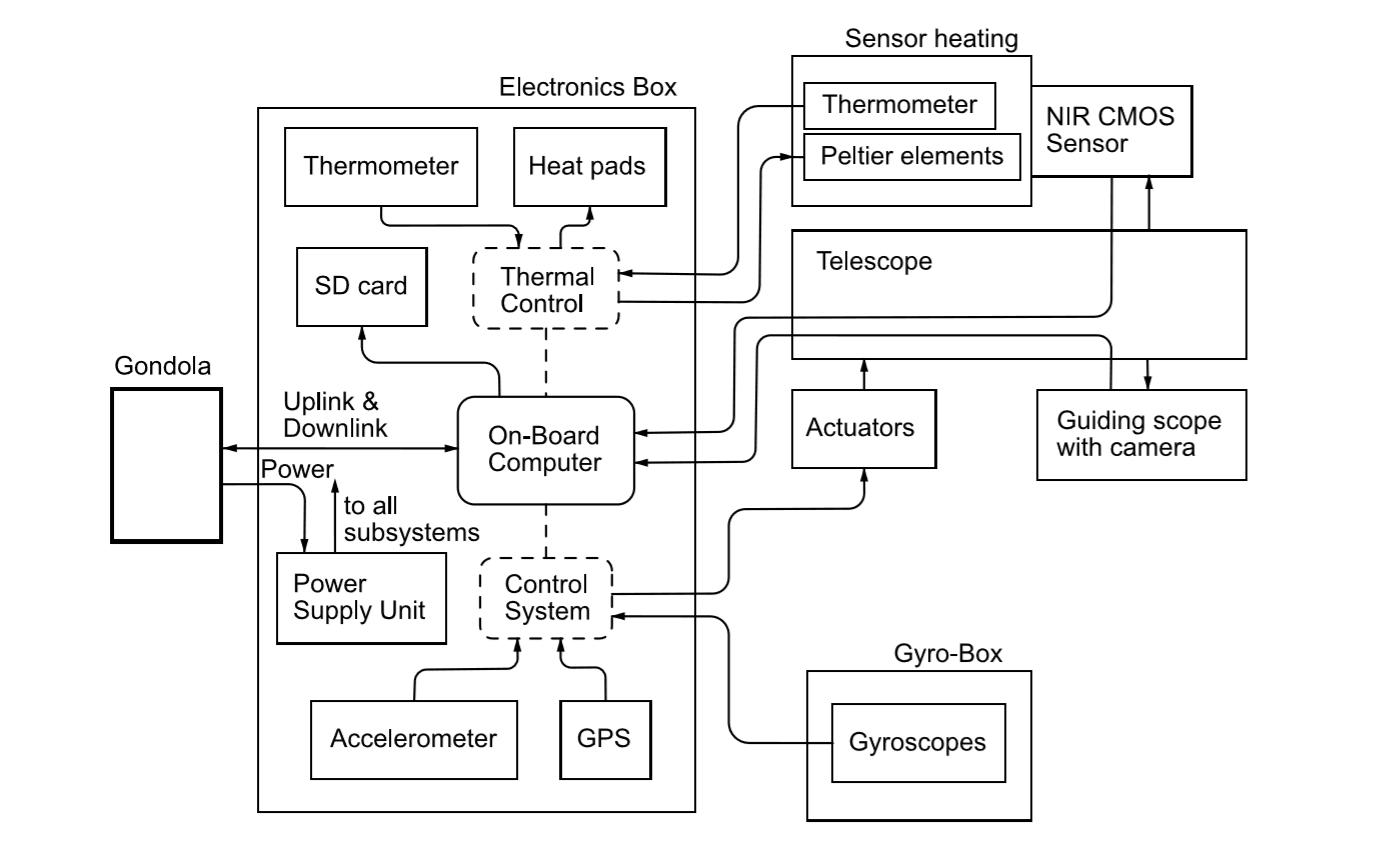
\includegraphics[width=.7\textwidth]{electrical/Setup.png}
           	\caption{Electrical setup}
        \end{figure}
    \end{frame}
    
	
	\begin{frame}[c]{Electrical - PCBs}
   	   \begin{itemize}
			\item PCB A: Power system, motor control and temperature actuator control
  			\item PCB B: Accelerometer, GPS, compass, temperature sensors
  			\item PCB C: Gyroscopes
       \end{itemize}
    \end{frame}
    
 	\begin{frame}[c]{Electrical - PCBs}
       \begin{figure}[H]
            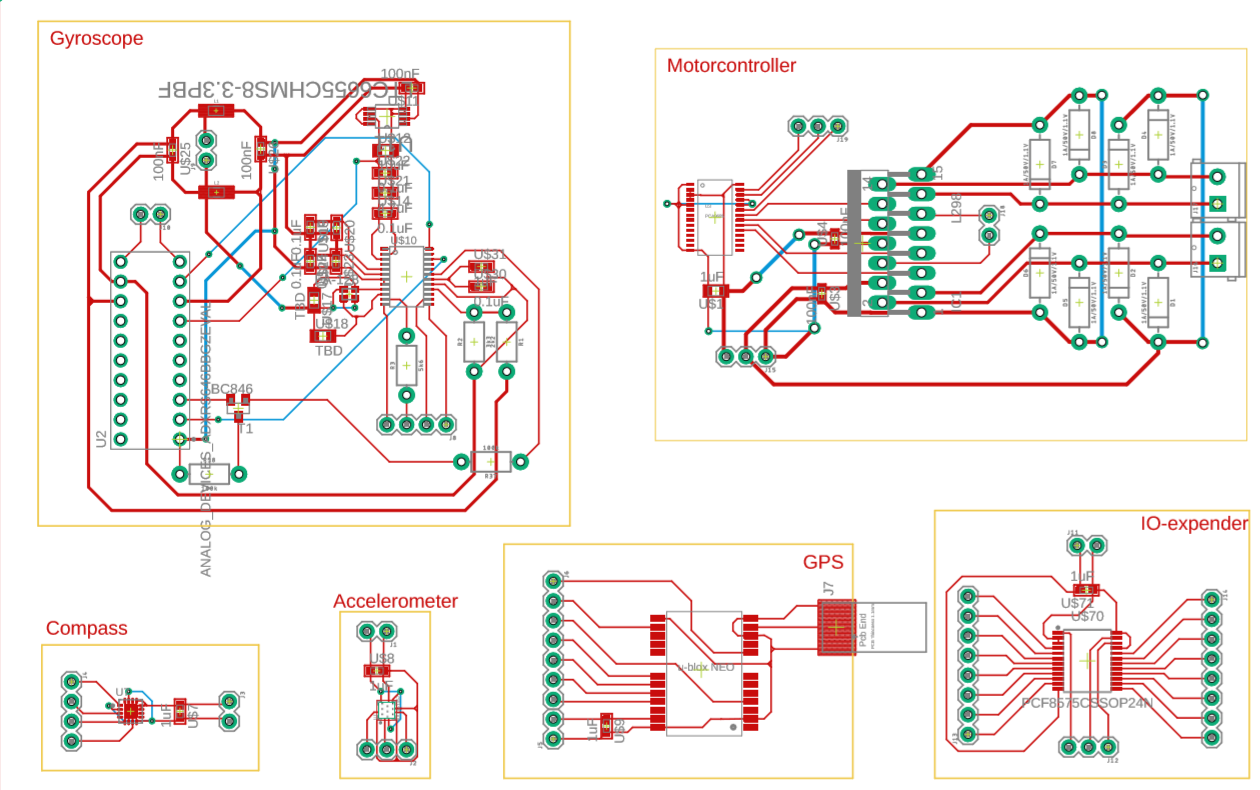
\includegraphics[width=.7\textwidth]{electrical/PCB_1st.png}
           	\caption{1st iteration of PCB design.}
        \end{figure}  
    \end{frame}

  	\begin{frame}[c]{Electrical - PCBs}
       \begin{figure}[H]
            \includegraphics[width=.7\textwidth]{electrical/GPStesting.png}
           	\caption{Testing of 1st iteration of PCB design.}
        \end{figure}  
    \end{frame}         

	\begin{frame}[c]{Electrical - Interfaces}
   		\begin{figure}
            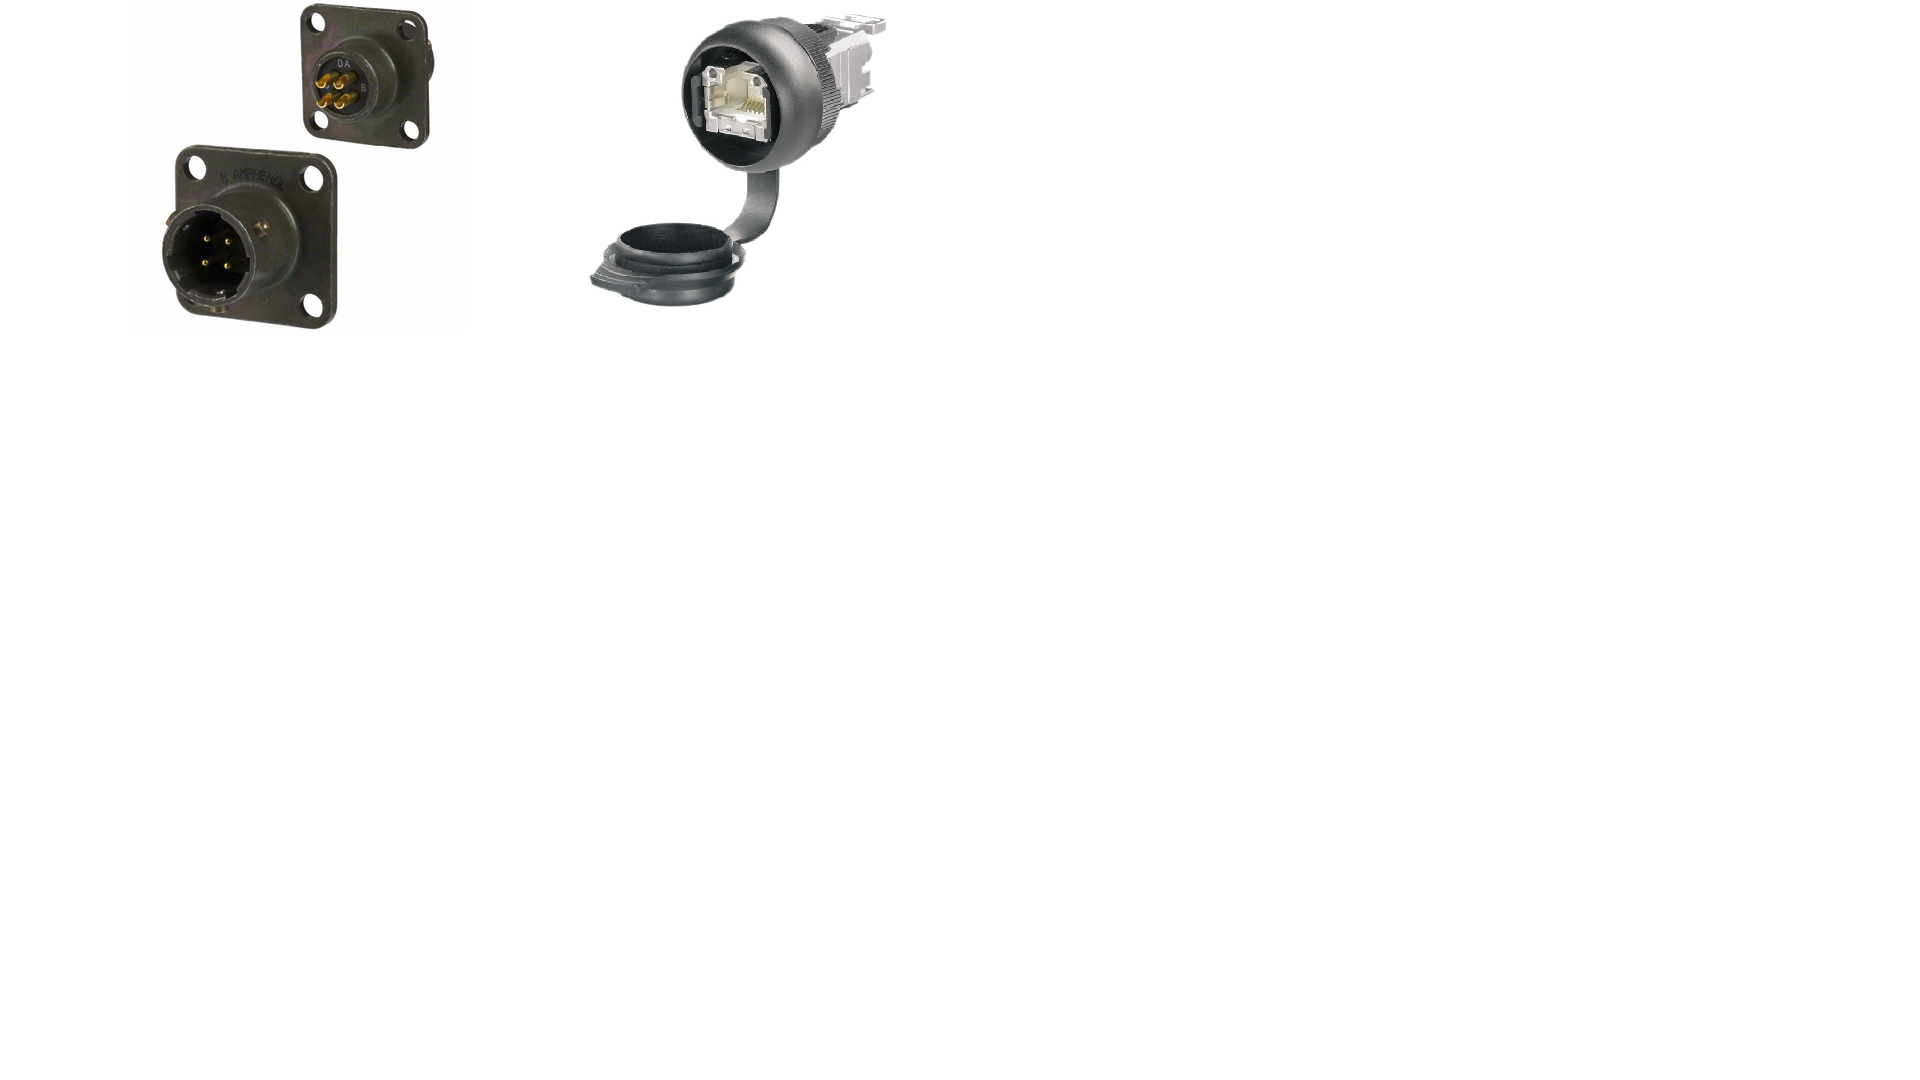
\includegraphics[width=.7\textwidth]{electrical/interface.png}
           	\caption{Figures from elfa.se.}
        \end{figure}
    \end{frame}
    

    
    \begin{frame}[c]{Electrical - Power}

 		\begin{figure}
           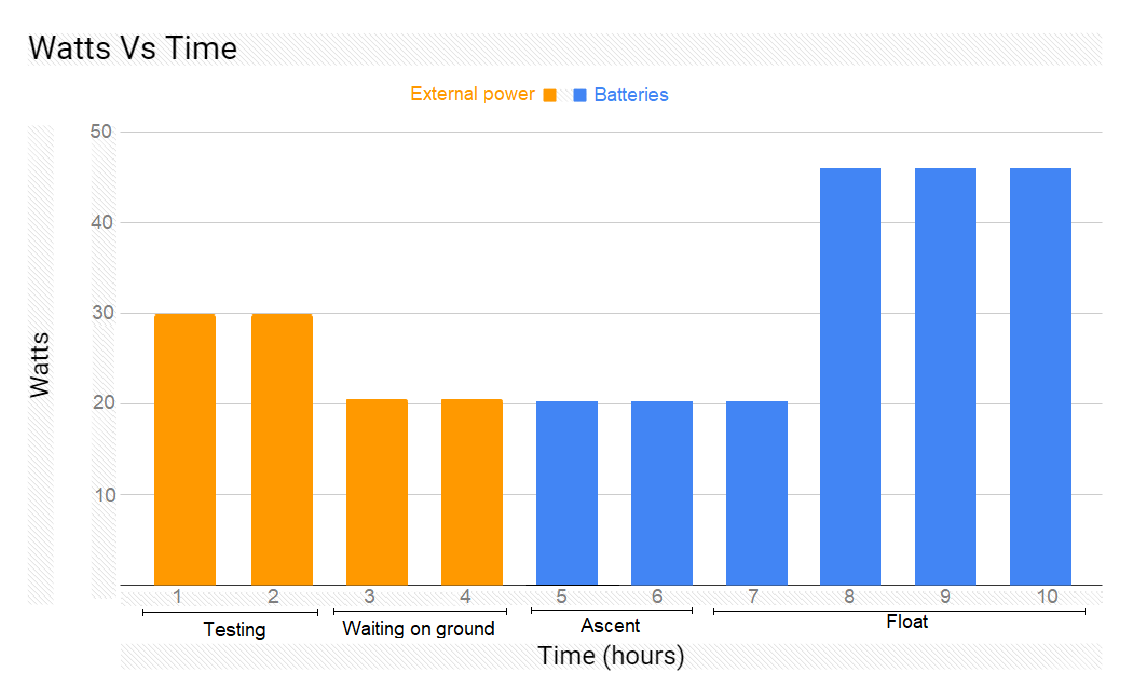
\includegraphics[width=.7\textwidth]{electrical/PowerDiagram.png}
           	
       	\end{figure} 
    
    \end{frame}

%   SOFTWARE. ---------------------------------------------------------------------------
\subsection{Software}

%%%%%%%%%%%%%%%%%%%%% states
    \begin{frame}[c]{Software - State Chart}
        \centering
        \begin{figure}
            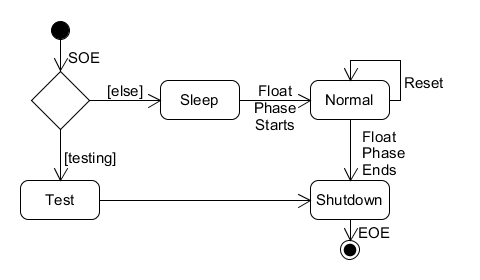
\includegraphics[width=.7\textwidth]{software/state-diagram.png}
        \end{figure}
    \end{frame}

%%%%%%%%%%%%%%%%%%%%% uplink
    \begin{frame}[c]{Software - E-link Uplink}

        \begin{columns}[t]
            \begin{column}{.5\textwidth}
                Basic commands:
                \begin{itemize}
                    \item Rebooting
                    \item Updating targets
                    \item Calibrating tracking
                    \item Controlling downlink
                    \item Setting camera settings
                    \item Guiding / Sanity
                    \item Mode transition
                \end{itemize}
            \end{column}

            \begin{column}{.5\textwidth}
                \only<2->{
                    \vspace{1cm}\\
                    \large{Maximum data rate:\\a few kbit/s}
                }
            \end{column}
        \end{columns}
    \end{frame}

%%%%%%%%%%%%%%%%%%%%% downlink
    \begin{frame}[t]{Software - E-link Downlink Load}
        \centering
        \vspace{1cm}
        \begin{center}
            \begin{tabular}{| l | l | l | l |}
                \hline
                \textbf{Item} & \textbf{File size} & \textbf{Downlink rate} & \textbf{Data rate} \\\hline\hline

                Guiding camera    & 2\,MB     & 60\,s / on request    & 270\,kbit/s  \\\hline
                NIR camera        & 20\,MB    & variable              & 440\,kbit/s  \\\hline
                Sanity camera     & 4\,MB     & on request            & -            \\\hline
                Sensors           & 100\,B    & 1\,s                  & 1\,kbit/s    \\\hline
            \end{tabular}
        \end{center}

        \only<2->{
            \vspace{.5cm}
            Minimum: 300\,kbit/s\quad Nominal: 500\,kbit/s
        }
    \end{frame}

%   GROUND STATION?. --------------------------------------------------------------------

    \begin{frame}[c]{Software - Ground Station}
        Role:
        \begin{itemize}
            \item Send telecommands
            \item Receive and display telemetry
        \end{itemize}
    \end{frame}

    \begin{frame}[c]{Software - Risks}
        \begin{itemize}
            \item Mode transitions
            \item Worst case scenario: SSH
        \end{itemize}
    \end{frame}

%   CONTROL. ----------------------------------------------------------------------------
\subsection{Control System}

\begin{frame}{Control system}
    Objectives of the control system:
    \begin{itemize}
        \item Selection and tracking the astronomical targets
        \item Stabilisation the telescope during exposure
        \item Avoid pointing the telescope at the Sun
        \item Thermal control of the CMOS sensor and the electronics box
    \end{itemize}
\end{frame}

\begin{frame}{Control system}
    \begin{itemize}
        \item<1-> Selection of targets: %\\
        \begin{itemize}
            \item Based on prioritisation parameters (e.\,g. brightness, location)
            \item Sensor data: star tracker, GPS %\\
        \end{itemize}
        \item<2-> Tracking of targets: 
        \begin{itemize}
            \item Model of movements of astronomical targets
            \item Sensor data: internal clock, GPS
        \end{itemize}
        \item<3-> Stabilisation of the gimbal: dynamic control system (PID) %\\
        \begin{itemize}
            \item Mechanical model of the gimbal, motors model
            \item Sensor data: gyroscopes, encoders%\\
        \end{itemize}
        \item<4-> Feedback loop, measured states: 
        \begin{itemize}
            \item Kalman filter determines exact position \& orientation
        \end{itemize}
    \end{itemize}
\end{frame}

\begin{frame}[c]{Control system}
    \begin{figure}
        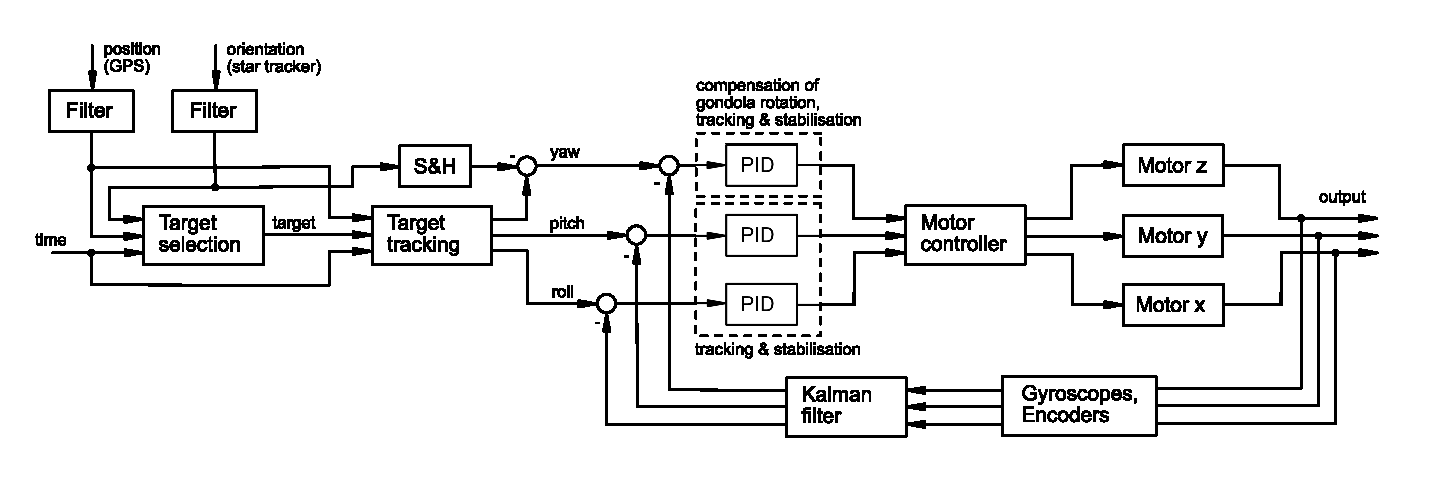
\includegraphics[width=\linewidth]{figures/images/Control_loop_v2.eps}
    \end{figure}
\end{frame}

\begin{frame}[c]{Control system - Risks}
    \begin{itemize}
        \item Not being able to choose appropriate PID values and R and Q matrices for the Kalman filter.\\
        \rotatebox[origin=c]{180}{$\Lsh$} Solutions: 
        \begin{itemize}
            \item Analytical approach
            \item Various tests on both model and prototype
            \item Consultation with our mentor, who's a specialist in control field
        \end{itemize}
    \end{itemize}
\end{frame}

\subsection{Telescope and Cameras}
\begin{frame}[c]{Telescope and Cameras}
    \begin{columns}
    \begin{column}{0.3\textwidth}
        \begin{figure}[c]
            \centering
            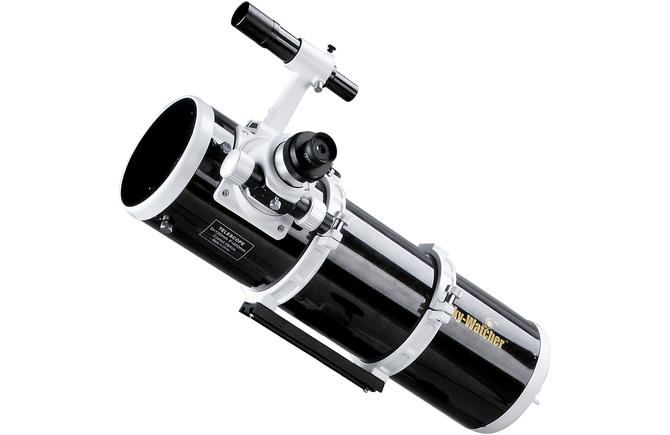
\includegraphics[width=\linewidth]{figures/images/SkyWatcher_BKP130DS.jpg}
            \caption*{SkyWatcher BKP 130DS (with eyepiece in place of the camera)}
        \end{figure}
    \end{column}
    \begin{column}{0.3\textwidth}
        \begin{figure}[c]
            \centering
            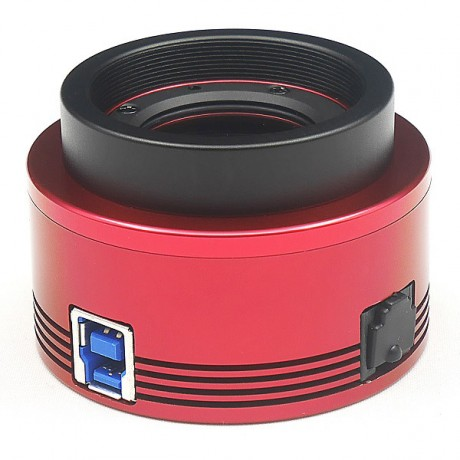
\includegraphics[width=\linewidth]{figures/images/ZWO_ASI183MM.jpg}
            \caption*{Credits: ZWO ASI183MM (mono)}
            % \label{fig::NIR_sensor}
        \end{figure}
    \end{column}
    \begin{column}{0.3\textwidth}
        \begin{figure}[c]
            \centering
            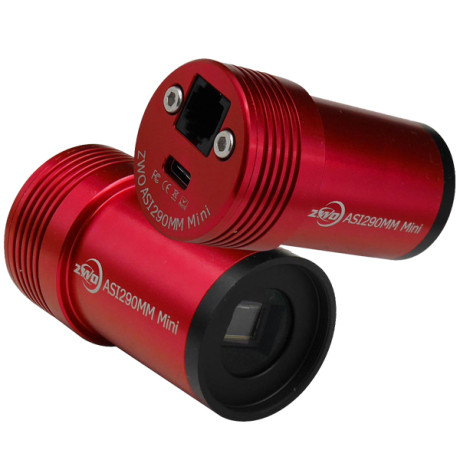
\includegraphics[width=\linewidth]{figures/images/ZWO_ASI290MM_Mini.jpg}
            \caption*{Credits: Guiding camera by ZWO}
            % \label{fig::guiding_camera}
        \end{figure}
    \end{column}
    \end{columns}
\end{frame}
%----------------------------------------------------------------------------------------
%   PROJECT MANAGEMENT.
%----------------------------------------------------------------------------------------
\section{Project Management}
%   TEAM. ---------------------------------------------------------------------------
\subsection{Team composition}
\begin{frame}[c]{Team composition}
    \begin{figure}
        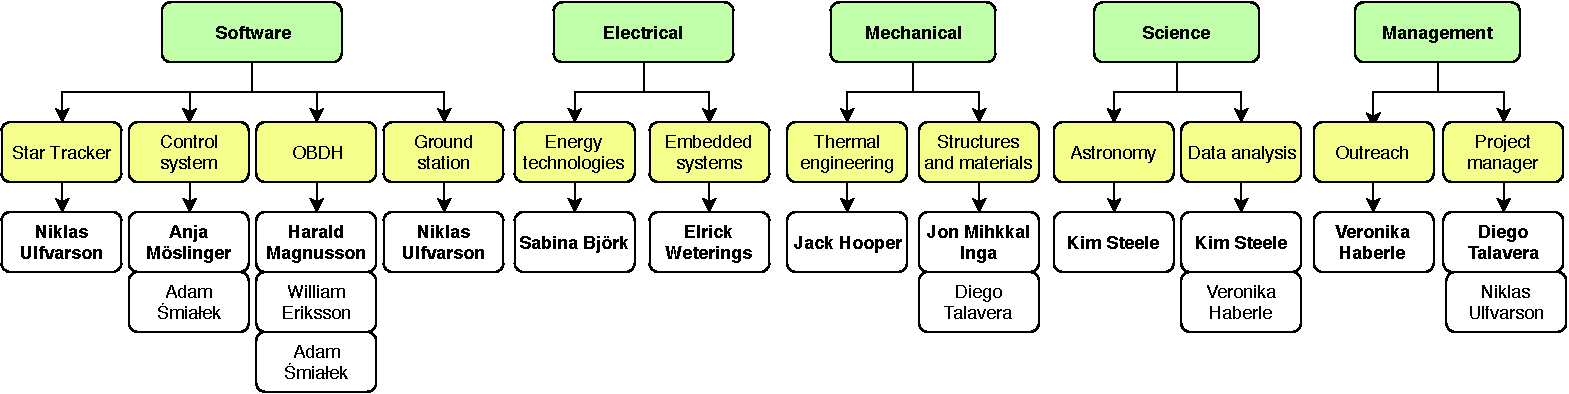
\includegraphics[width=\linewidth]{images/Team_structure.pdf}
        % \caption{Work breakdown structure}
    \end{figure}
\end{frame}

%   PLANNING. ---------------------------------------------------------------------------
\subsection{Project schedule}
\begin{frame}{Project schedule}
    \begin{figure}
        \vspace{-.1cm}
        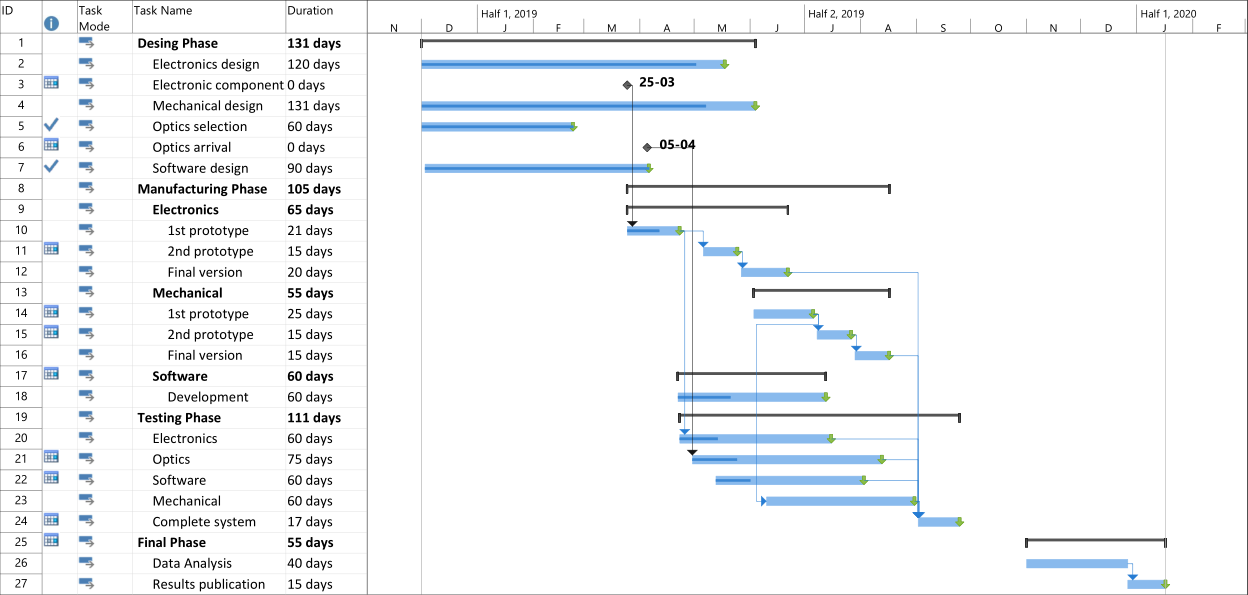
\includegraphics[height=0.9\textheight]{images/gantt.png}
    \end{figure}
\end{frame}

%   BUDGET. -----------------------------------------------------------------------------
\subsection{Budget}

\begin{frame}[c]{Budget (Expenses)}
    \centering
    \footnotesize
    \begin{tabular}{|l|c|c|c|} 
        \hline
        Component & Qty & Cost/Unit (\euro) & Cost (\euro)  \\ 
        \hline
        \rowcolor{Gray}
        \textbf{Structure} &  & \textbf{Total} & \textbf{590}  \\
        Bearings & TBD & TBD & 200 \\ 
        \hline
        \rowcolor{Gray}
        \textbf{Electronics} &  & \textbf{Total} & \textbf{631.5}  \\
        Motors & 3 & 21.99 & 66.0  \\
        Encoders & 2 & 44.2 & 88.4  \\
        GPS Receiver & 3 & 22.0 & 66.0  \\
        Various small components & n/a & n/a & 100  \\
        \hline
        
        \rowcolor{Gray}
        \textbf{Optical} &  & \textbf{Total} & \textbf{1420.5}  \\
        Telescope & 1 & 250.5 & 250.5  \\
        IR Camera & 1 & 800 & 800  \\
        Guiding Camera & 1 & 320 & 320  \\
        \hline
        
        \rowcolor{Gray}
        \textbf{Other} &  & \textbf{Total} & \textbf{1300}  \\
        Error margin & n/a & n/a & 250  \\
        Travel PDR/CDR & 2 & 500 & 1000 \\
        \hline
        \textbf{Total projected cost} &  &  & \textbf{3942}  \\
        \hline
    \end{tabular}
\end{frame}

\begin{frame}[c]{Budget (Funding)}
    \centering
    \small
    \begin{tabular}{|l|c|c|} 
        \hline
        Source & Amount (\euro) & Limitations   \\ 
        \hline
        Luleå University of Technology & $\approx2500$ & Hardware and travel \\
        SNSA & $\approx3000$ & Hardware and travel \\
        Crowdfunding Campaign & TBD & None \\
        \hline
        \textbf{Total projected income} & \textbf{$\approx5500$} & \\
        \hline
        \bf{Total projected cost} & \bf{3942} & \\
        \hline
    \end{tabular}
\end{frame}
    
    %   OUTREACH. ---------------------------------------------------------------------------
\subsection{Outreach}

\begin{frame}[c]{Outreach}
    \begin{minipage}[c]{0.40\linewidth}
        Published articles:
        \begin{itemize}
            \item Mölndals posten
        \end{itemize}
        Social media:        
        \begin{itemize}
            \item Website
            \item Facebook, Instagram and Twitter
        \end{itemize}
        Planned:
        \begin{itemize}
            \item University and high school Presentations
            \item Local newspapers articles
        \end{itemize}
    \end{minipage}
    \begin{minipage}[c]{0.30\linewidth}
        \begin{figure}[]
            \centering
            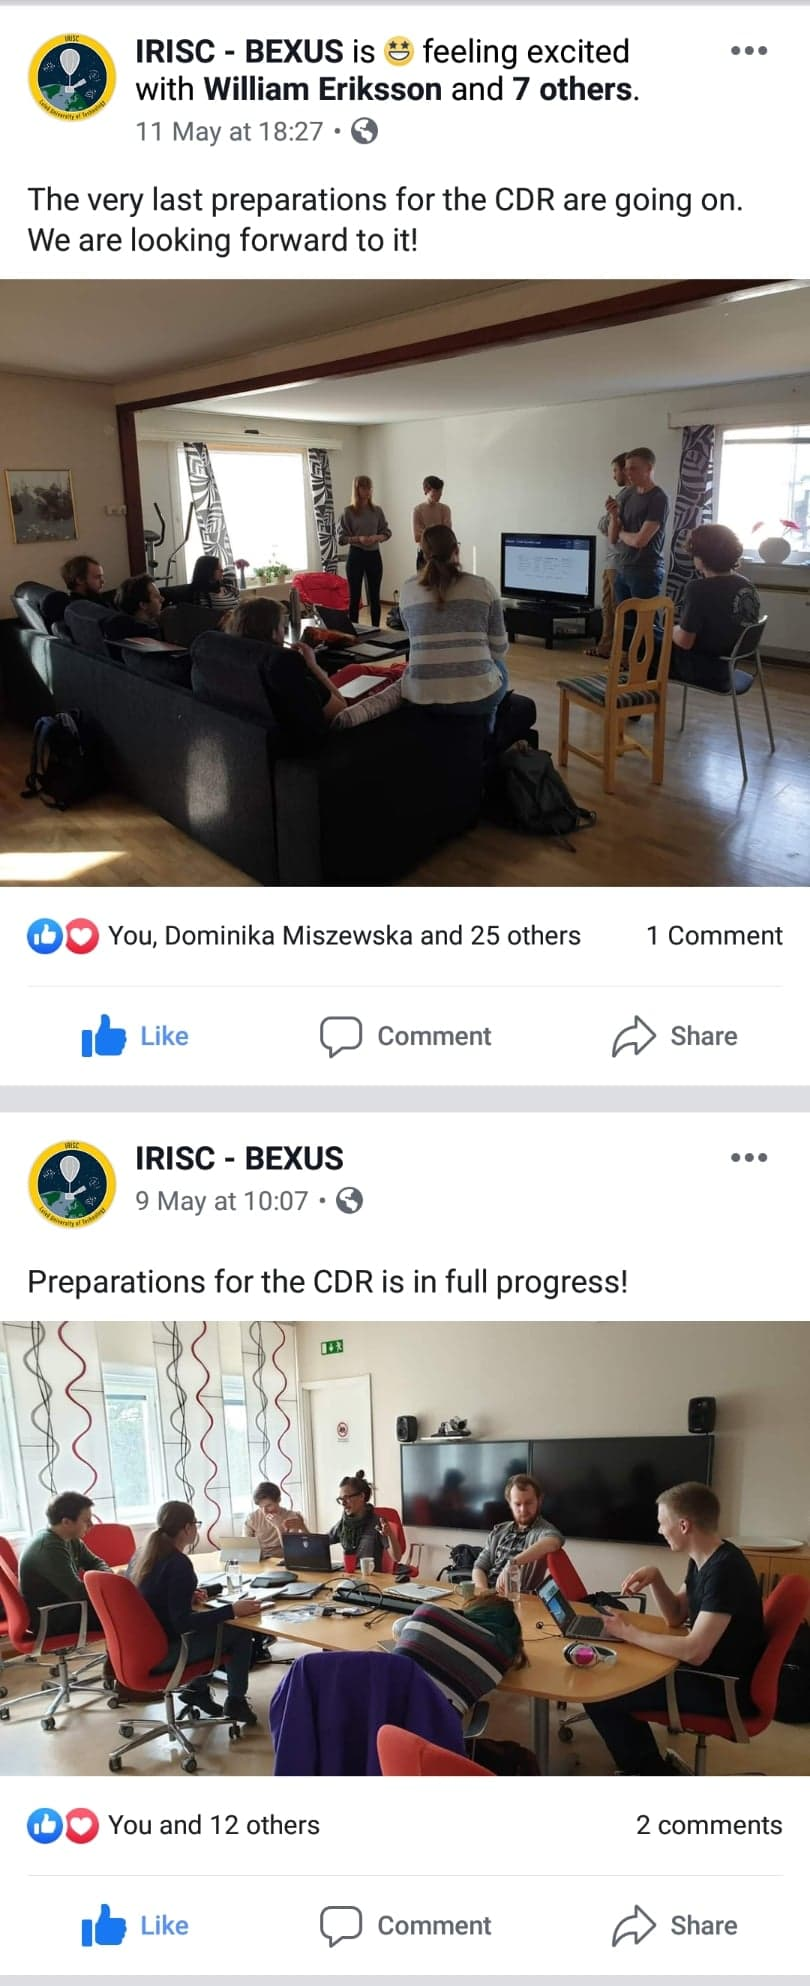
\includegraphics[height=0.9\textheight]{images/facebook.jpg}
            \label{}
        \end{figure}
    \end{minipage}
    \begin{minipage}[c]{0.25\linewidth}
        \begin{figure}[]
            \centering
            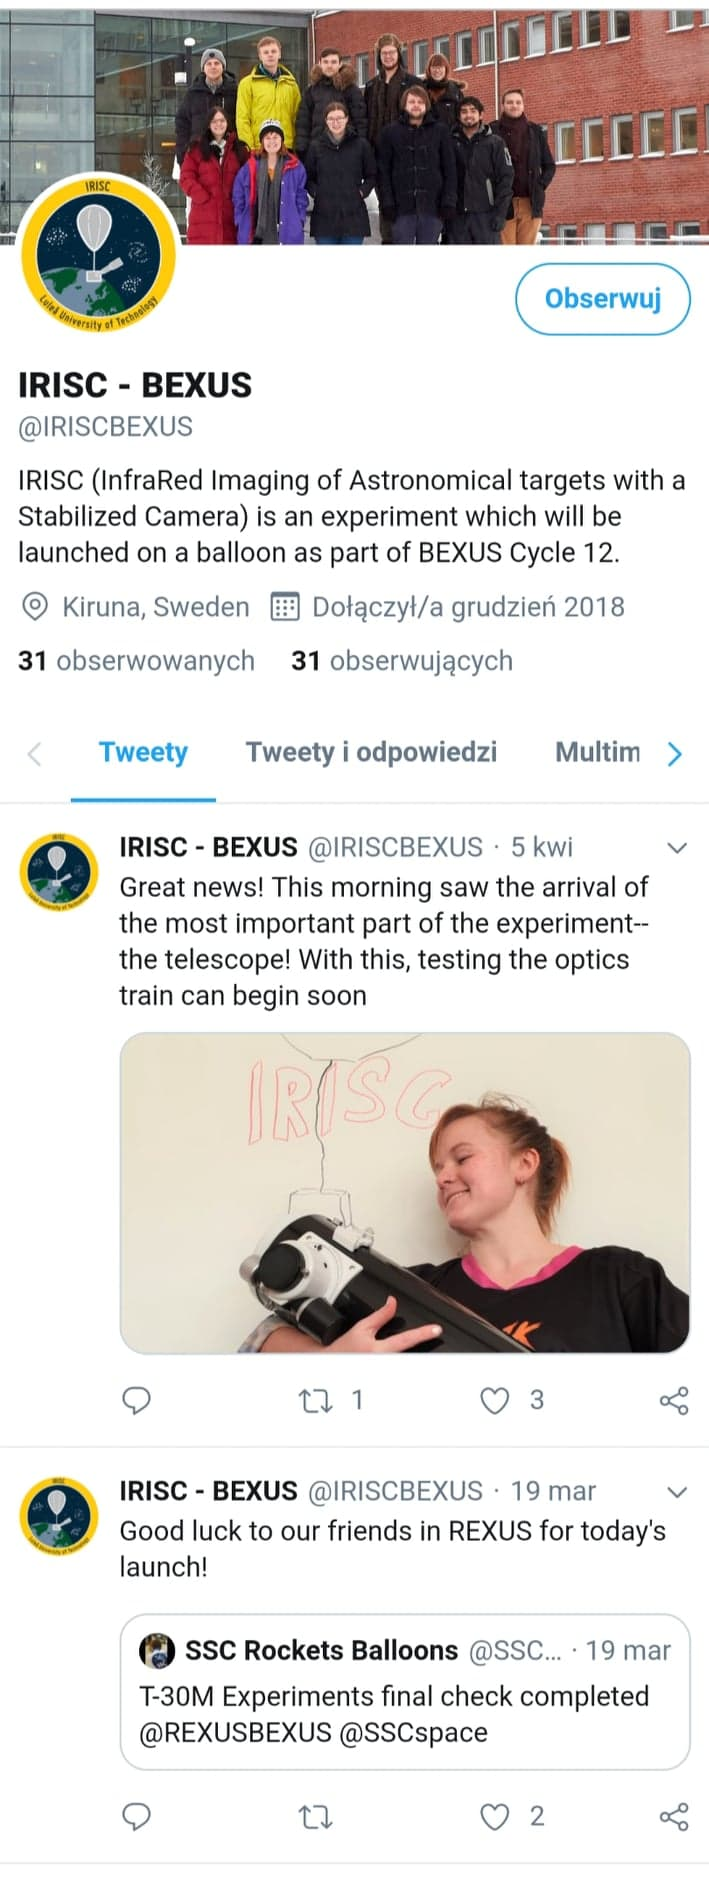
\includegraphics[height=0.9\textheight]{images/twitter.jpg}
            \label{}
        \end{figure}
    \end{minipage}
\end{frame}


%----------------------------------------------------------------------------------------
%   SUMMARY.
%----------------------------------------------------------------------------------------
\section{Summary}

%----------------------------------------------------------------------------------------
%   QUESTIONS.
%----------------------------------------------------------------------------------------
\section{Questions}

%\begin{frame}[plain]{}
%%    \label{slide:questions}
%%    \centering
%%    \vspace{-0.71cm}
%%    \begin{figure}
%%    \hspace*{-1.1cm}
%%      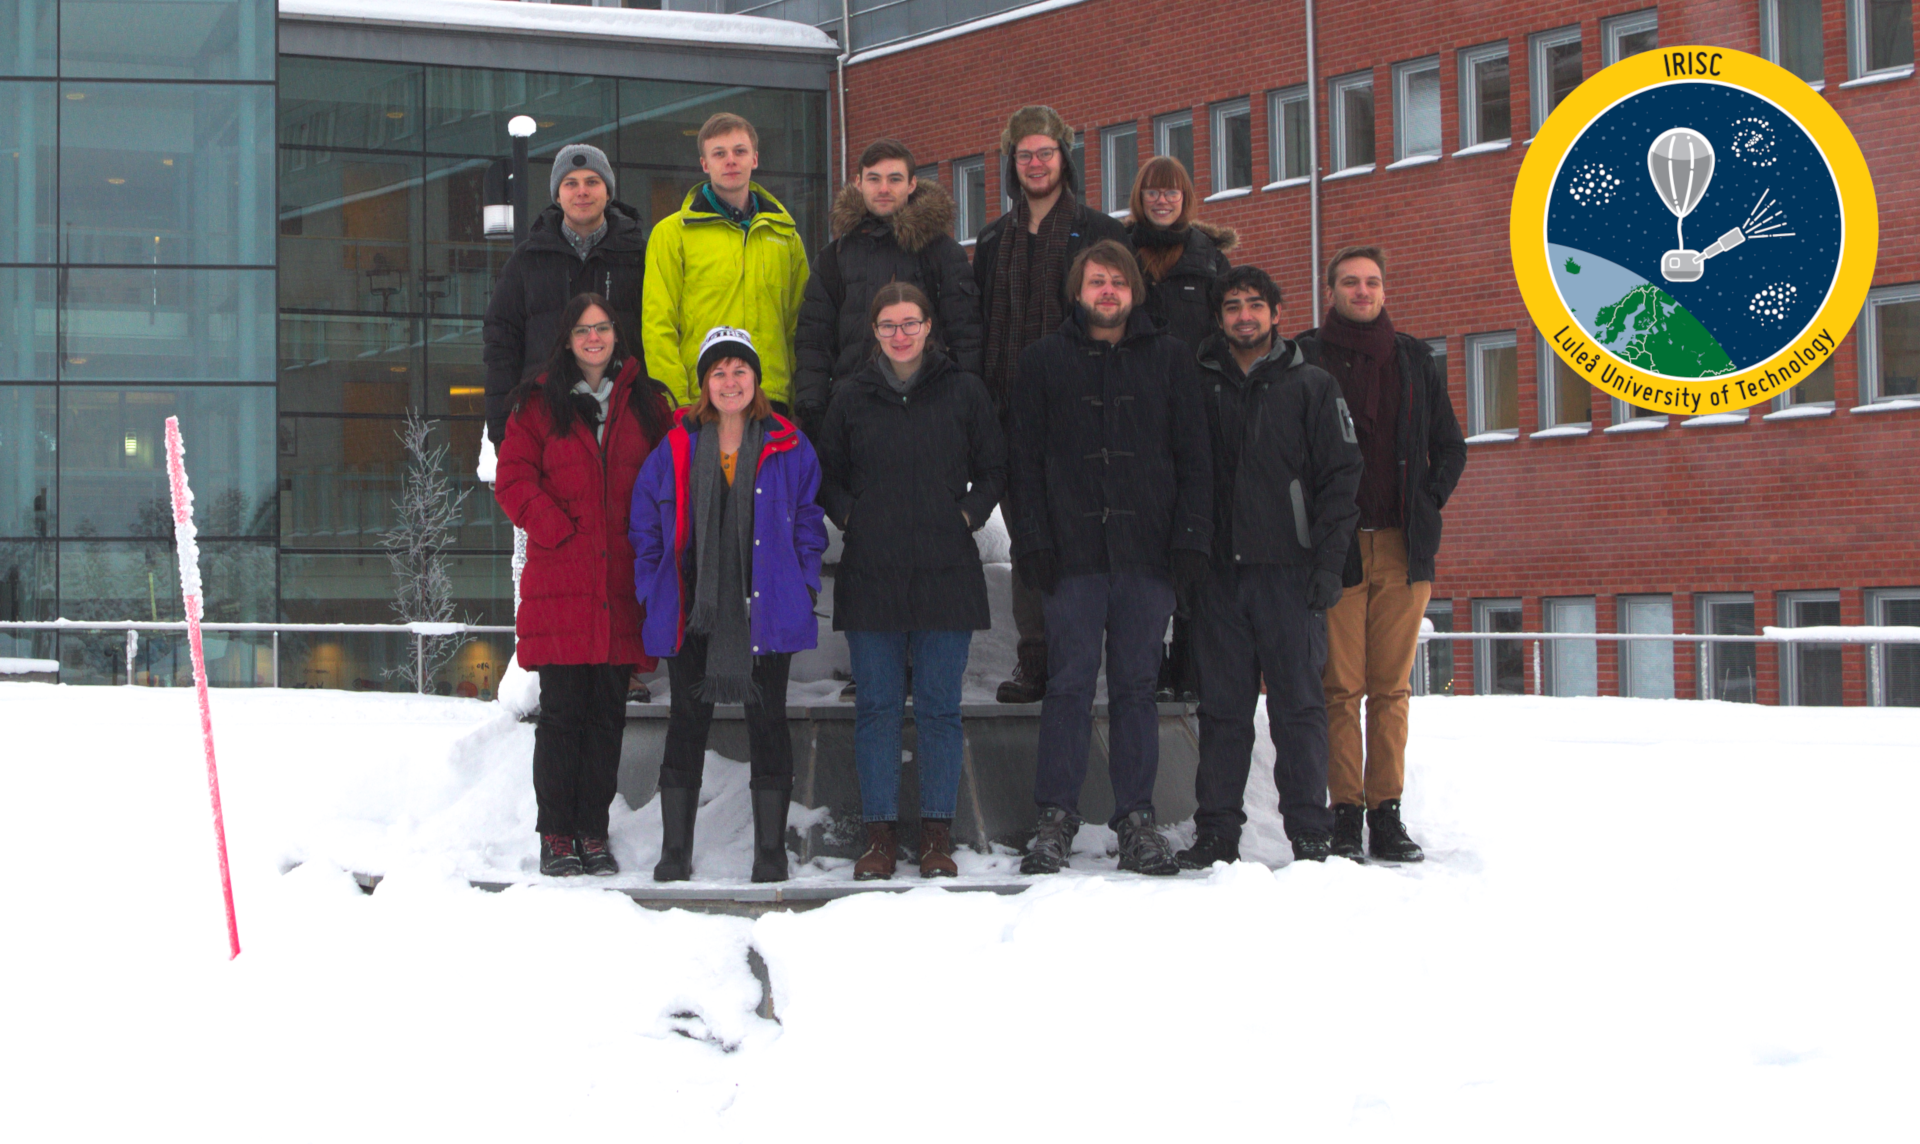
\includegraphics[width=1.15\textwidth]{figures/images/teamphoto.png}
%%    \end{figure}
%   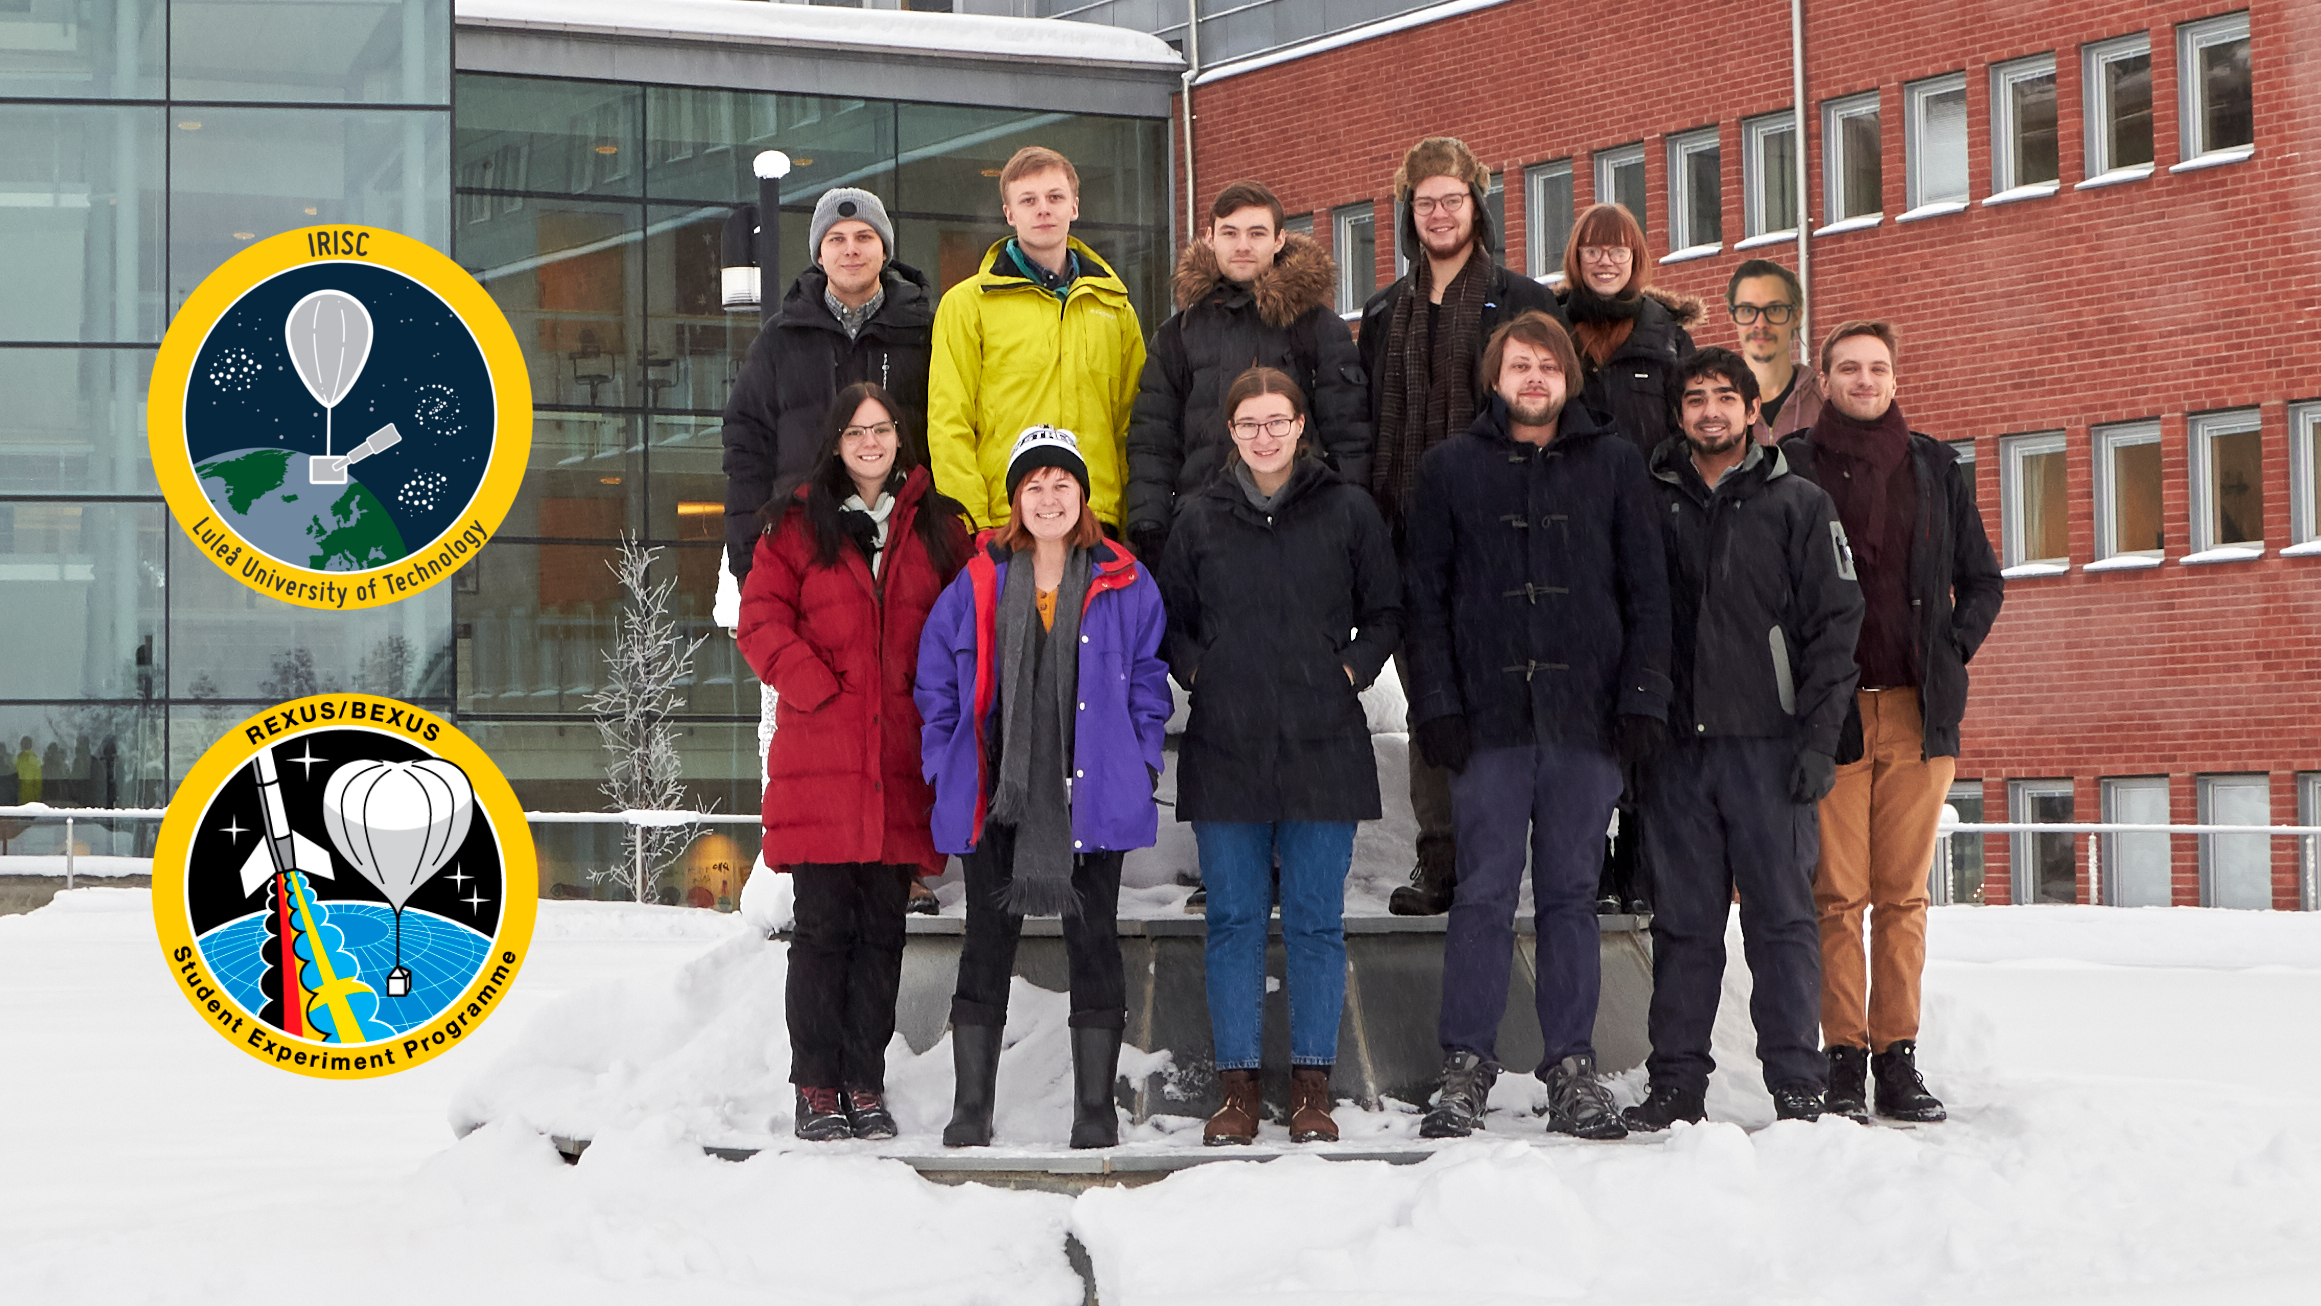
\includegraphics[width=\paperwidth]{figures/images/IRISC_Team_001_16_9+logo.jpg}
%\end{frame}
{
\usebackgroundtemplate{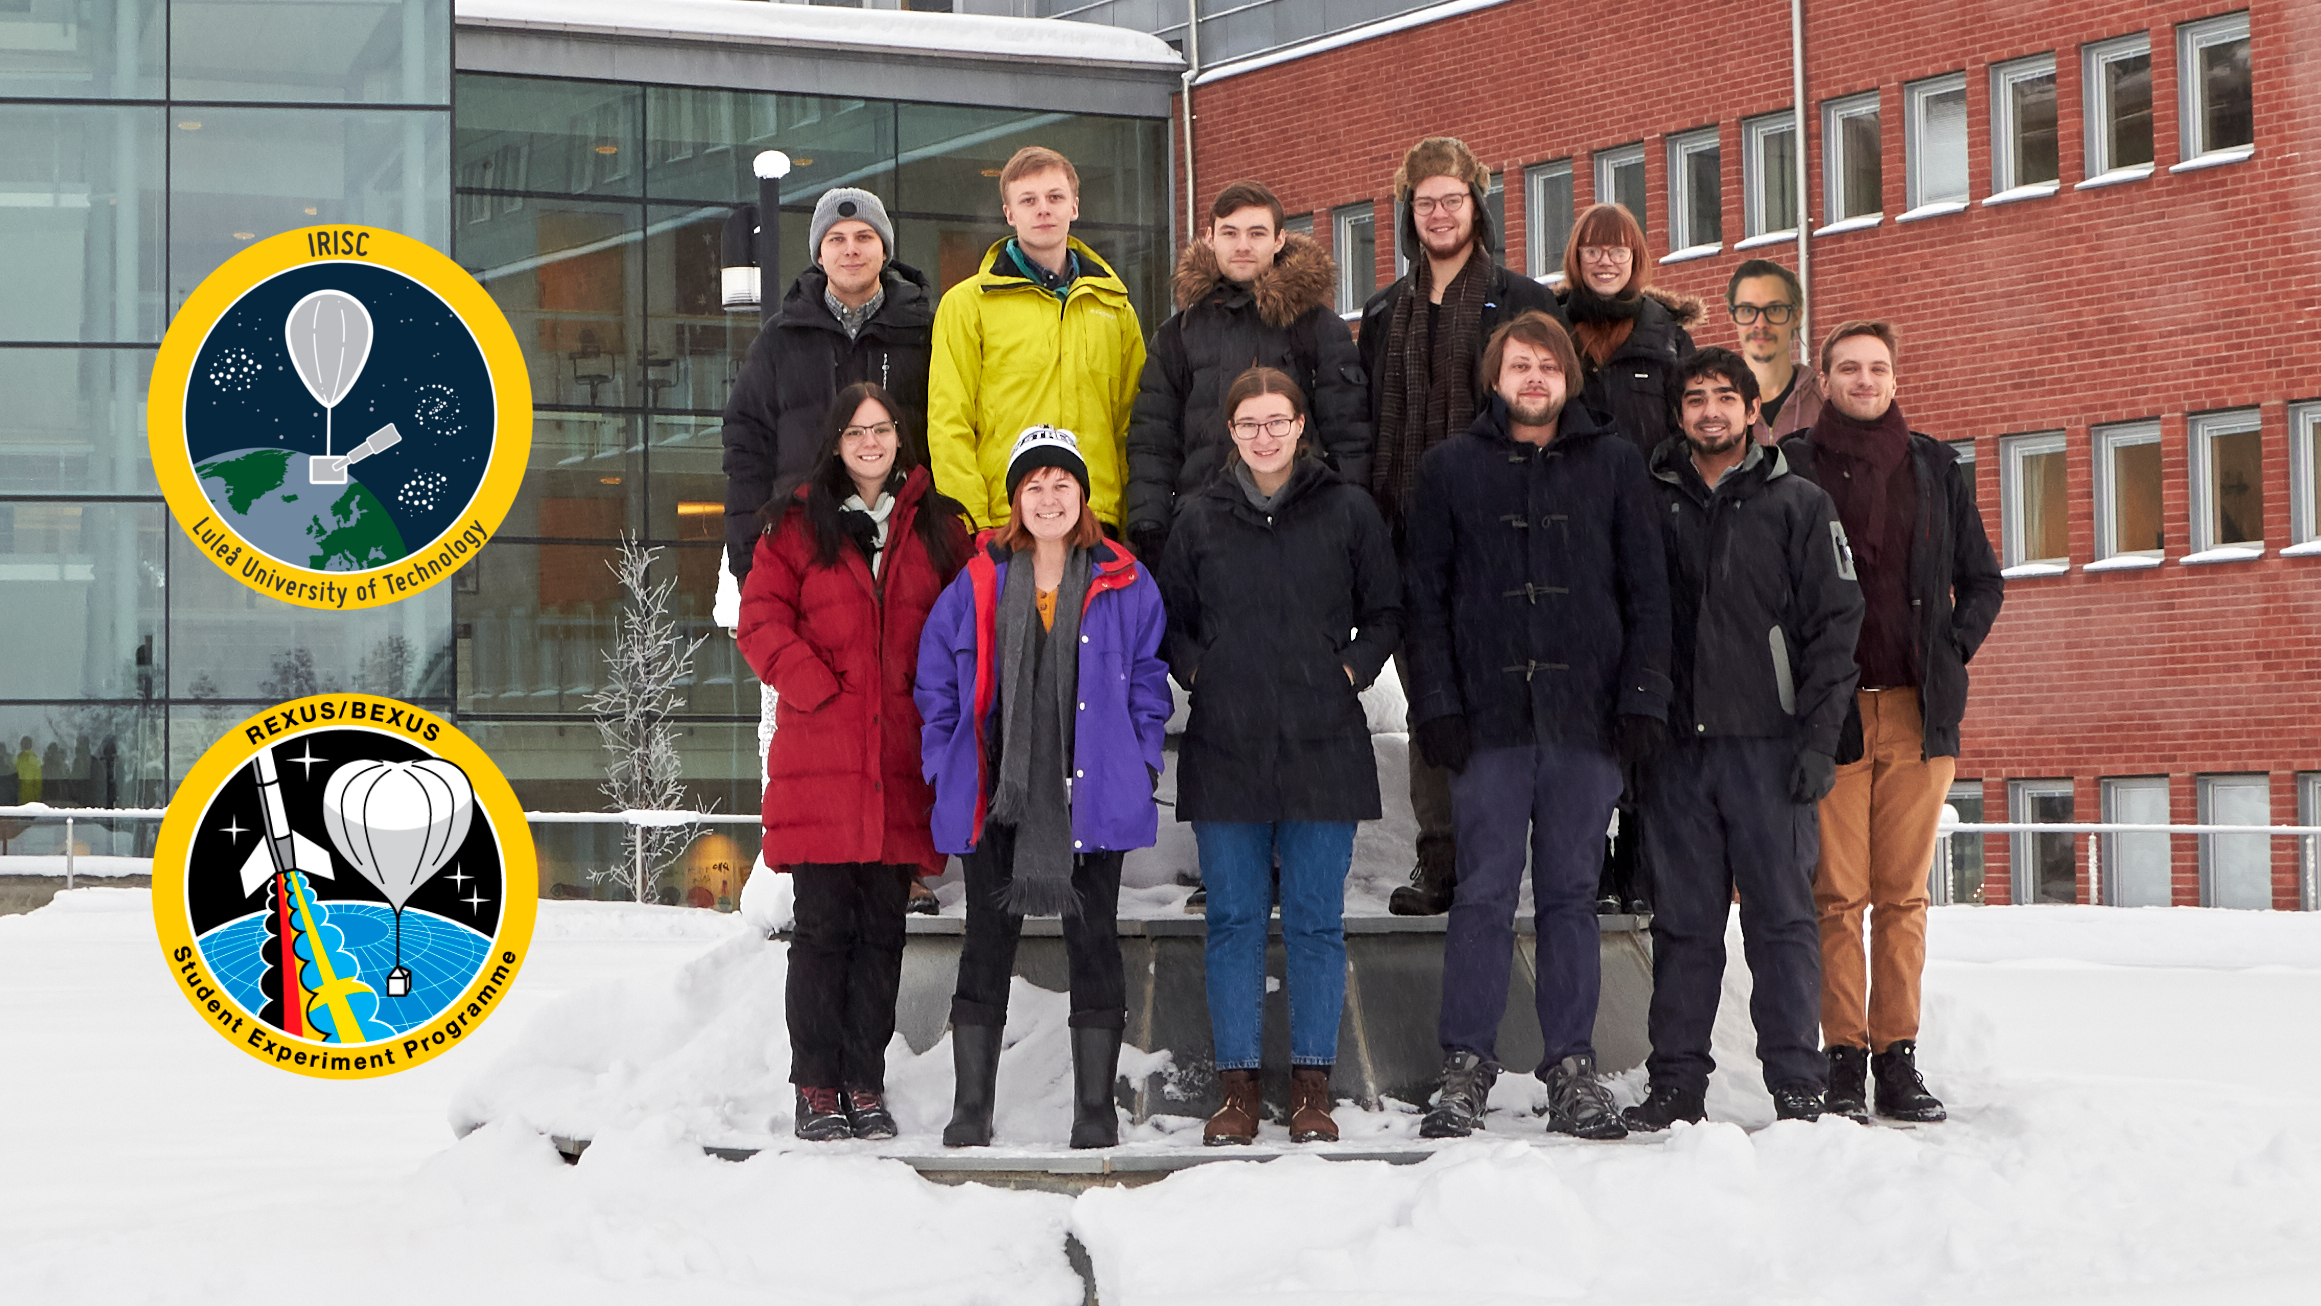
\includegraphics[width=\paperwidth]{figures/images/IRISC_Team_001_16_9+logo.jpg}}
\begin{frame}[plain]
\label{slide:questions}
\end{frame}

}
%----------------------------------------------------------------------------------------
%   BACKUP SLIDES.              EVERYONE!!!
%----------------------------------------------------------------------------------------

%  Software
%----------------------------------------------------------------------------------------

%%%%%%%%%%%%%%%%%%%%% process overview
\begin{frame}[c]{Software - Interface Overview}
    \begin{figure}
        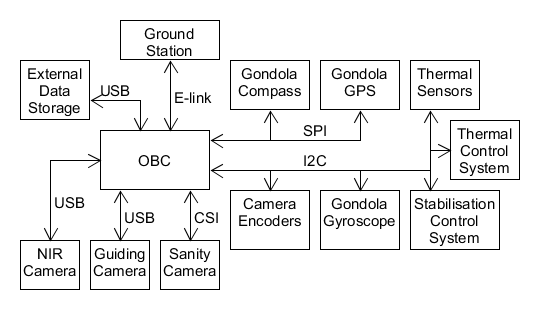
\includegraphics[height=\textheight]{software/process-overview.png}
    \end{figure}
\end{frame}

%%%%%%%%%%%%%%%%%%%%% composition
\begin{frame}[c]{Software - Composition}
    \begin{figure}
        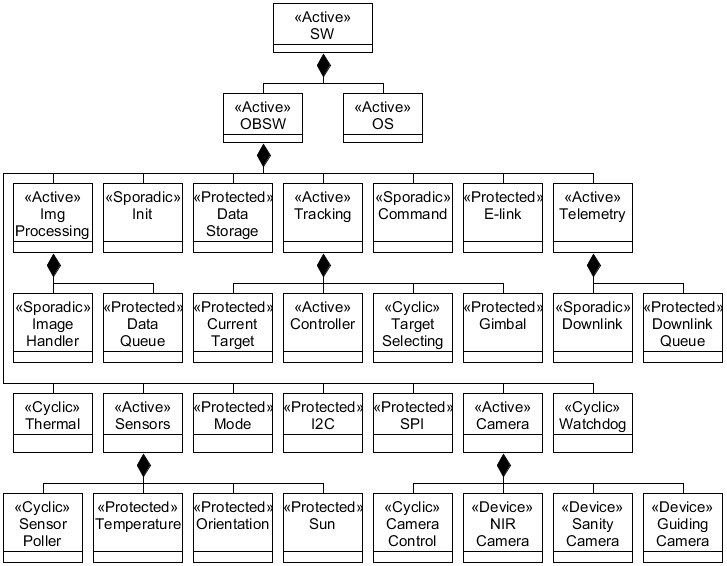
\includegraphics[height=.9\textheight]{software/composition-tree.png}
    \end{figure}
\end{frame}

%%%%%%%%%%%%%%%%%%%%% flow
\begin{frame}[c]{Software - Activity}
    \centering
    \begin{columns}[t]
        \begin{column}{.5\textwidth}
            \vspace{1cm}\\
            Low activity ``sleep'' during ascent\\
            \vspace{1cm}
                Switch conditions:
                \begin{itemize}
                    \item Target leaves operational field of view
                    \item A higher priority target enters the field of view
                \end{itemize}
        \end{column}

        \begin{column}{.5\textwidth}
            \vspace{-1 cm}
            \begin{figure}
                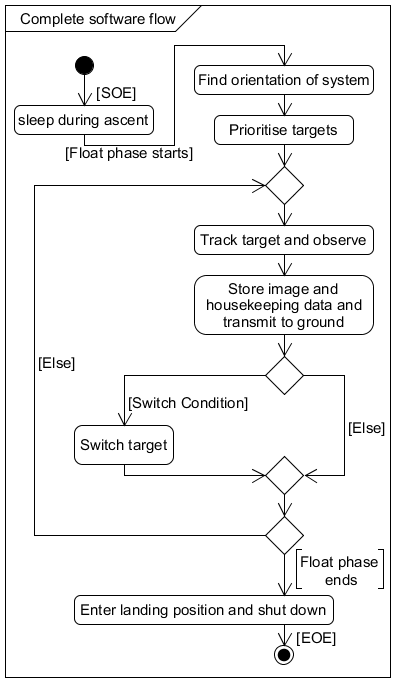
\includegraphics[height=.9\textheight]{software/activity-diagram.png}
            \end{figure}
        \end{column}
    \end{columns}
\end{frame}


%%%%%%%%%%%%%%%%%%%%% relations tree
\begin{frame}[c]{Software - Relations Tree}
    \begin{figure}
        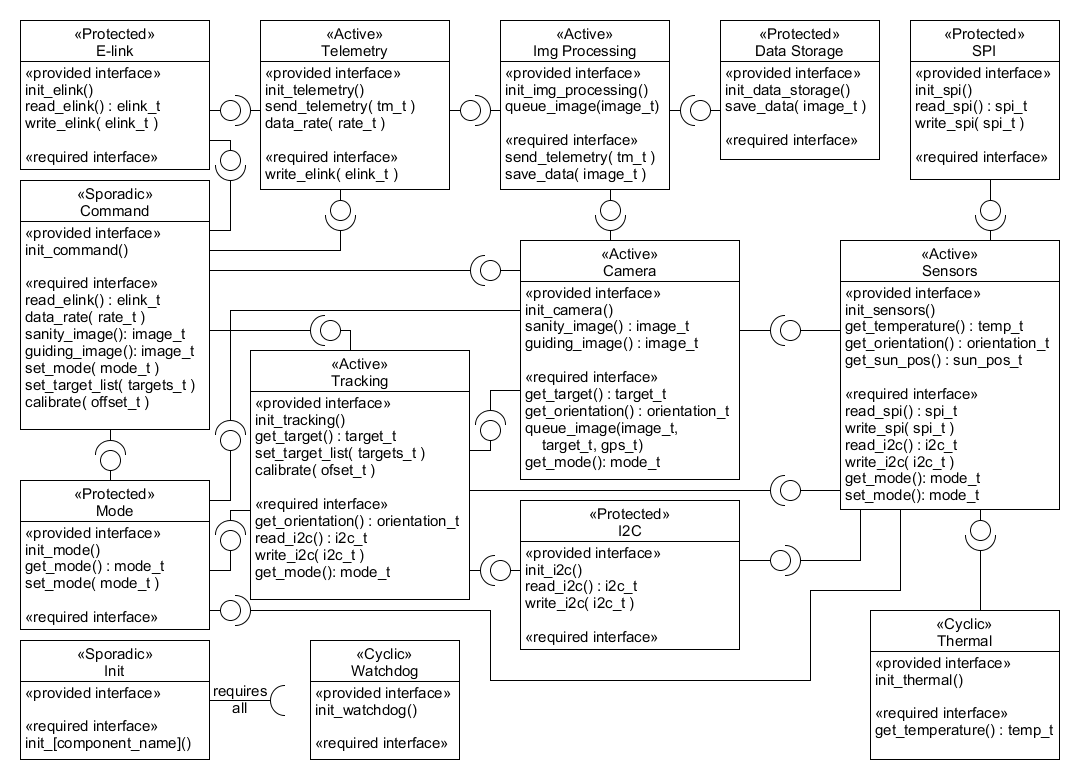
\includegraphics[height=.9\textheight]{software/complete_relations_tree.png}
    \end{figure}
\end{frame}

%  END Software
%----------------------------------------------------------------------------------------
\begin{frame}[c]{Thermal control loop}
    \begin{figure}
        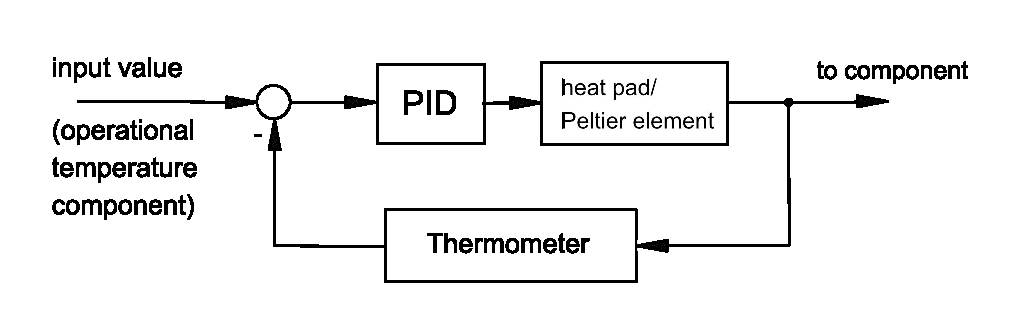
\includegraphics[width=\textwidth]{figures/images/Thermal_control.eps}
        \caption*{Thermal control loop}
    \end{figure}
\end{frame}

\begin{frame}
    \frametitle{Control system resolutions}
    \begin{itemize}
        \item 
    \end{itemize}
\end{frame}

\begin{frame}{Budget (1)}
    \centering
    \begin{tabular}{|l|c|c|c|} 
        \hline
        Component & Qty & Cost/Unit (\euro) & Cost (\euro)  \\ 
        \hline
        \rowcolor{Gray}
        \textbf{Structure} &  &  & \textbf{590}  \\
        Aluminium profile, 20x20mm & 3000 mm & n/a & 20  \\
        Aluminium profile, 30x30mm & 2000 mm & n/a & 35  \\
        M6 T-bolt & 30 & 0.9 & 27  \\
        M4 T-slot & 2 & 7.5 & 15  \\
        90-deg connector, 20mm & 8 & 3.1 & 25 \\
        90-deg connector, 30mm & 10 & 5 & 50 \\
        Aluminium sheet, 1mm & 500x500mm & n/a & 20 \\
        Aluminium sheet, 2mm & 500x500mm & n/a & 70 \\
        Bearings & TBD & TBD & 200 \\
        Tools & n/a & n/a & 78 \\
        Various small components & n/a & n/a & 50  \\
        \hline
    \end{tabular}
\end{frame}
\begin{frame}{Budget (2)}
    \centering
    \begin{tabular}{|l|c|c|c|} 
        \hline
        Component & Qty & Cost/Unit (\euro) & Cost (\euro)  \\ 
        \hline
        \rowcolor{Gray}
        \textbf{Electronics (part 1)} &  &  & \textbf{631.5}  \\ 
        Raspberry Pi 3 B+ & 1 & 29.5 & 29.5  \\
        Raspberry Pi Zero & 1 & 22.6 & 22.6  \\
        Peltier element & 1 & 35.2 & 35.2  \\
        Heating pad & 1 & 17.7 & 17.7  \\ 
        Motors & 3 & 21.99 & 66.0  \\ 
        Motor controller & 1 & 4.7 & 4.7  \\
        Encoders & 2 & 44.2 & 88.4  \\
        GPS Receiver & 3 & 22.0 & 66.0  \\ 
        GPS Antenna & 1 & 17.2 & 17.2  \\
        Gyroscope & 1 & 54.2 & 54.2  \\
        \hline
    \end{tabular}
\end{frame}
\begin{frame}{Budget (3)}
    \centering
    \begin{tabular}{|l|c|c|c|} 
        \hline
        Component & Qty & Cost/Unit (\euro) & Cost (\euro)  \\ 
        \hline
        \rowcolor{Gray}
        \textbf{Electronics (part 2)} &  &  & \textbf{631.5}  \\ 
        Raspberry Pi Camera V2 & 1 & 23.6 & 23.6  \\ 
        ADC & 1 & 18.3 & 18.3  \\ 
        ADC & 1 & 4.8 & 4.8  \\
        SD-card 32GB & 2 & 21.5 & 43  \\
        SD-card 8GB & 1 & 6.5 & 6.5  \\
        U-regulator & 1 & 10.6 & 10.6  \\
        Various small components & n/a & n/a & 100  \\
        \hline
    \end{tabular}
\end{frame}
\begin{frame}{Budget (4)}
    \centering
    \begin{tabular}{|l|c|c|c|} 
        \hline
        Component & Qty & Cost/Unit (\euro) & Cost (\euro)  \\ 
        \hline
        \rowcolor{Gray}
        \textbf{Optical} &  &  & \textbf{1420.5}  \\
        Telescope & 1 & 250.5 & 250.5  \\
        IR Camera & 1 & 800 & 800  \\
        Guiding Camera & 1 & 320 & 320  \\
        Camera mounting adapter & 1 & 50 & 50 \\
        \hline
        \rowcolor{Gray}
        \textbf{Other} &  &  & \textbf{1300}  \\
        Shipping costs & n/a & n/a & 50  \\
        Error margin & n/a & n/a & 250  \\
        Travel PDR/CDR & 2 & 500 & 1000 \\
        \hline
        \textbf{Total} &  &  & \textbf{3942}  \\
        \hline
    \end{tabular}
\end{frame}

%   CAMERA. -----------------------------------------------------------------------------
\begin{frame}{NIR Camera for the telescope}
    \vspace{-0.2cm}
    \begin{columns}[t]
    \begin{column}{0.6\textwidth}
        \begin{itemize}
            \item CMOS Sensor: ZWO ASI183MM (mono-colour) \\
                resolution: 20.18\,MP, sensor size: 13.2x8.8\,mm
            \item NIR-conversion with 720\,nm NIR filter
            %\item Sensitivity: 720\,nm to 1150\,nm
            \item Rolling shutter: no mechanical shutter, no moving parts
        \end{itemize}
        \vspace{-0.7cm}
        \begin{figure}
        \centering
        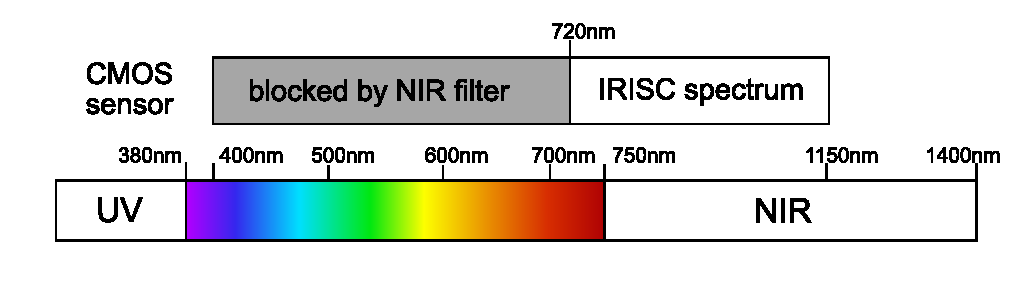
\includegraphics[width = 1.1\linewidth]{figures/images/IRISC_spectrum.eps}
    \end{figure}
    \end{column}
    \begin{column}{0.4\textwidth}
        \begin{figure}[t]
            \centering
            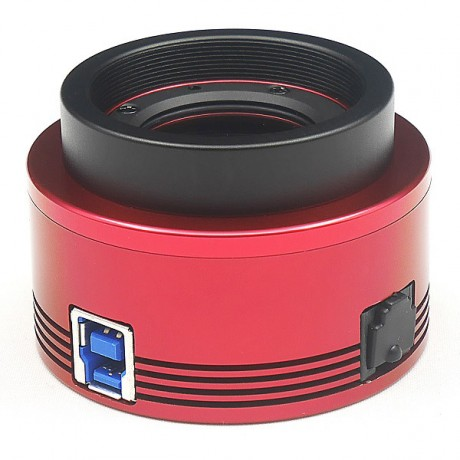
\includegraphics[width=0.7\linewidth]{figures/images/ZWO_ASI183MM.jpg}
            \caption*{Credits: ZWO ASI183MM (mono)}
            \label{fig::NIR_sensor}
        \end{figure}
    \end{column}
    \end{columns}
\end{frame}

\begin{frame}{Guiding Camera}
    \begin{columns}[t]
    \begin{column}{0.6\textwidth}
    \begin{itemize}
        \item For verification of the field of view (7.5\,deg)
        \item Support of ground-based re-calibration of sensors (e.\,g.~magnetometer, gyroscopes)
        \item Imaging sensor with a high sensitivity, resulting in shorter exposure times (compared to NIR camera)
        \item Imaging in visible wavelengths and NIR
    \end{itemize}

    \end{column}
    \begin{column}{0.4\textwidth}
        \begin{figure}[t]
            \centering
            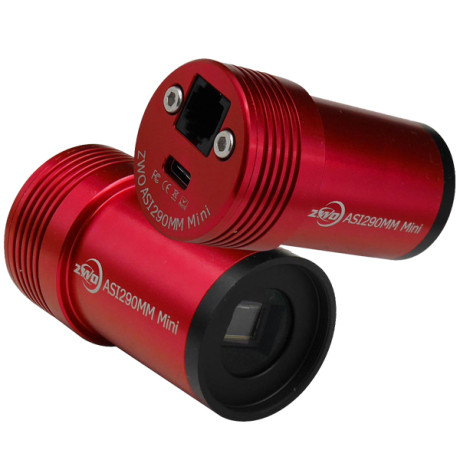
\includegraphics[width=0.7\linewidth]{figures/images/ZWO_ASI290MM_Mini.jpg}
            \caption*{Credits: Guiding camera by ZWO}
            \label{fig::guiding_camera}
        \end{figure}
    \end{column}
    \end{columns}
\end{frame}

\begin{frame}{Telescope}
    \begin{figure}[!htb]
        \centering
        \begin{minipage}{.5\textwidth}
            \centering
            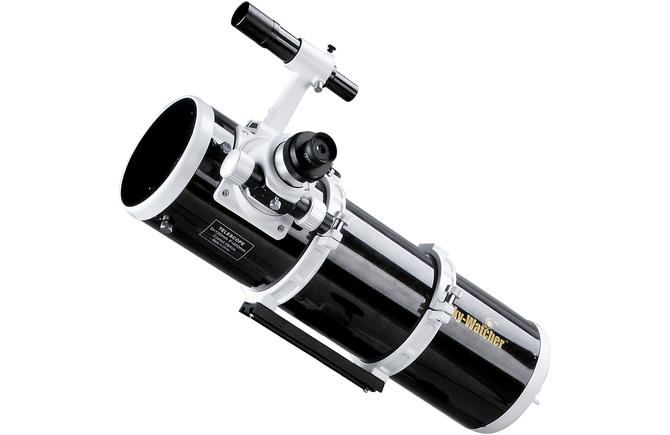
\includegraphics[width=\linewidth]{figures/images/SkyWatcher_BKP130DS.jpg}
            \caption*{SkyWatcher BKP 130DS (with eyepiece in place of the camera)}
        \end{minipage}%
        \begin{minipage}{0.5\textwidth}
            SkyWatcher BKP 130DS
            \begin{itemize}%[label=--]
                \item Newtonian telescope
                \item Focal length: 650\,mm
                \item Aperture: 130\,mm
                \item FOV: 1.16\,deg by 0.78\,deg
                \item Diffraction-limited-resolution: 1.94\,arcsec
                \item Pixel size: 0.76\,arcsec (in \newline combination with the camera)    
            \end{itemize}
        \end{minipage}
    \end{figure}
\end{frame}

\begin{frame}[t]{Targets (brightness-ordered)}
    \begin{table}[]
        \tiny
        \begin{tabular}{|c|c|c|c|c|c|c|}
            \hline
            \textbf{Name}                  & \textbf{Designation} & \textbf{RA}    & \textbf{DEC}    & \textbf{Mag}  & \textbf{Dim x (arcsec)} & \textbf{Dim y (arcsec)} \\ \hline
            Andromeda Galaxy      & M31         & 0.70  & 41.27  & 3.44 & 190   & 60    \\ \hline
            Open Star Cluster     & M52         & 23.40 & 61.58  & 5    & 13    & 13    \\ \hline
            Reflection Nebula     & NGC 1333    & 3.48  & 31.35  & 5.6  & 6     & 3     \\ \hline
            Triangulum galaxy     & M33         & 1.55  & 30.65  & 5.72 & 70.8  & 41.7  \\ \hline
            Hercules Globular     & M13         & 16.68 & 36.45  & 5.8  & 20    & 20    \\ \hline
            Eagle Nebula          & M16         & 18.30 & -12.18 & 6    & 7     & 7     \\ \hline
            Iris Nebula           & NGC 7023    & 21.02 & 68.17  & 6.8  & 18    & 18    \\ \hline
            Veil Nebula           & NGC 6992    & 20.75 & 30.70  & 7    & 180   & 180   \\ \hline
            The Wizard Nebula     & NGC 7380    & 22.78 & 58.10  & 7.2  & 25    & 25    \\ \hline
            Pacman Nebula         & NGC 281     & 0.87  & 56.62  & 7.4  & 20    & 30    \\ \hline
            Starfish Open Cluster & M38         & 5.47  & 35.85  & 7.4  & 21    & 21    \\ \hline
            Crescent Nebula       & NGC 6888    & 20.20 & 38.35  & 7.4  & 18    & 12    \\ \hline
            Dumbbell Nebula       & M27         & 19.98 & 22.72  & 7.5  & 8     & 5.6   \\ \hline
            Pinwheel galaxy       & M101        & 14.05 & 54.33  & 7.8  & 28.8  & 26.9  \\ \hline
            Whirlpool Galaxy      & M51         & 13.48 & 47.18  & 8.4  & 11.2  & 6.9   \\ \hline
            Cigar Galaxy          & M82         & 9.92  & 69.67  & 8.41 & 11.2  & 4.3   \\ \hline
            Intergalactic Tramp   & NGC 2419    & 7.63  & 38.87  & 9.06 & 6     & 6     \\ \hline
            Sunflower galaxy      & M63         & 13.25 & 42.02  & 9.3  & 12.6  & 7.2   \\ \hline
            Bubble Nebula         & NGC 7635    & 23.33 & 61.20  & 10   & 15    & 8     \\ \hline
        \end{tabular}
    \end{table}
\end{frame}

----------------------------------------------------------------
% Electrical 


    \begin{frame}[c]{Electrical - Setup}
   		\begin{figure}[H]
            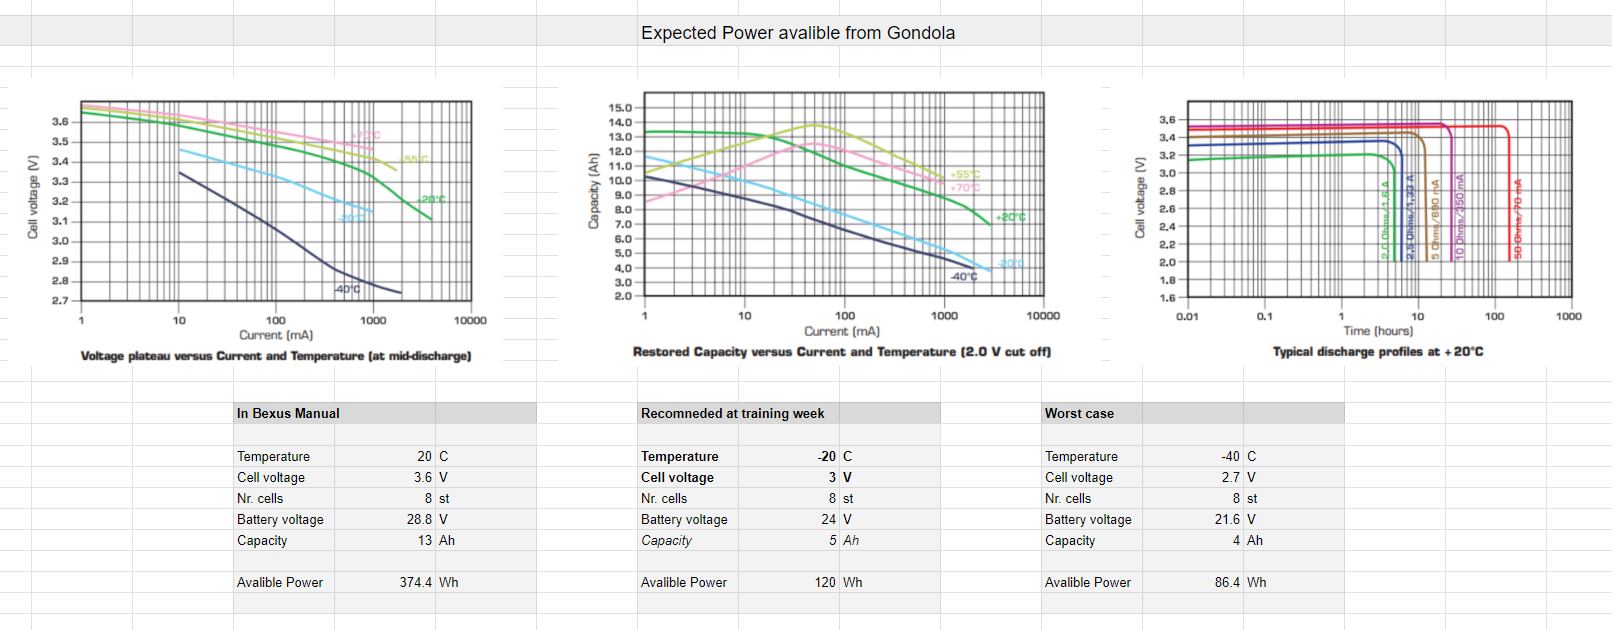
\includegraphics[width=.6\textwidth]{electrical/Backup-avaliblePower.png}
           	\caption{Avalible Power on gondola estimation, figure from Bexus Manual}
        \end{figure}
    \end{frame}
    
    
    \begin{frame}[c]{Electrical - Setup}
   		\begin{figure}[H]
            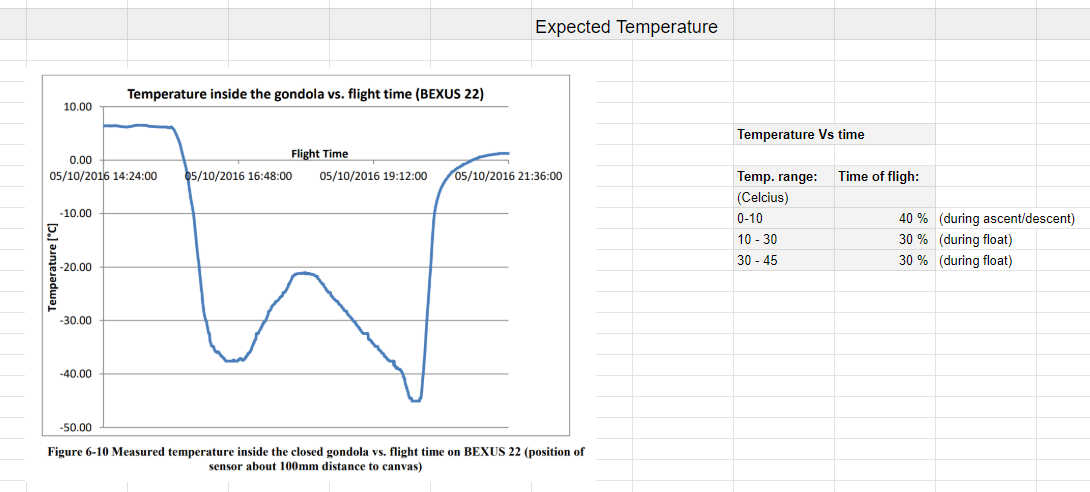
\includegraphics[width=.6\textwidth]{electrical/Backup-bexus22temp.png}
           	\caption{Bexus 22 temperature inside gondola, figure from Bexus Manual}
        \end{figure}
    \end{frame}

    \begin{frame}[c]{Electrical - Setup}
   		\begin{figure}[H]
            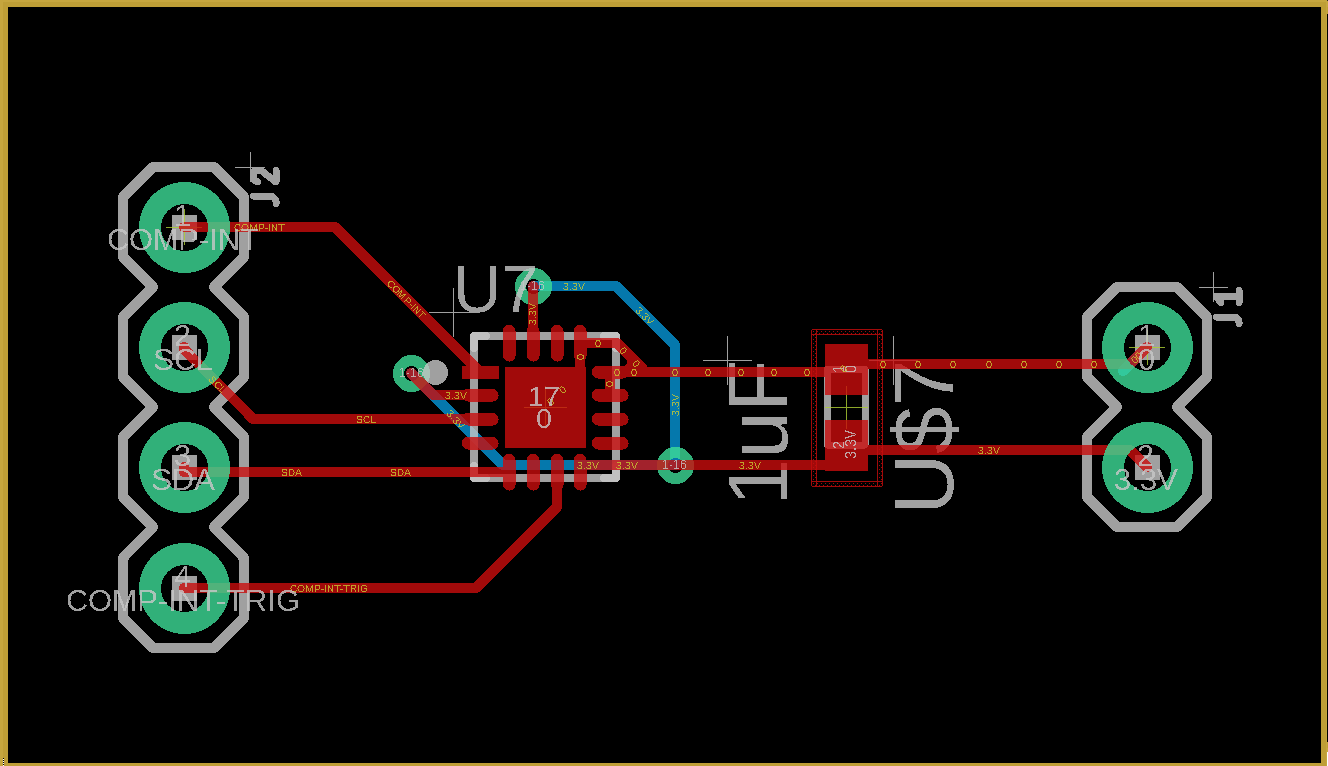
\includegraphics[width=.6\textwidth]{electrical/PCB_compass.png}
           	\caption{PCB 1st iteration : Compass}
        \end{figure}
    \end{frame}


    \begin{frame}[c]{Electrical - Setup}
   		\begin{figure}[H]
            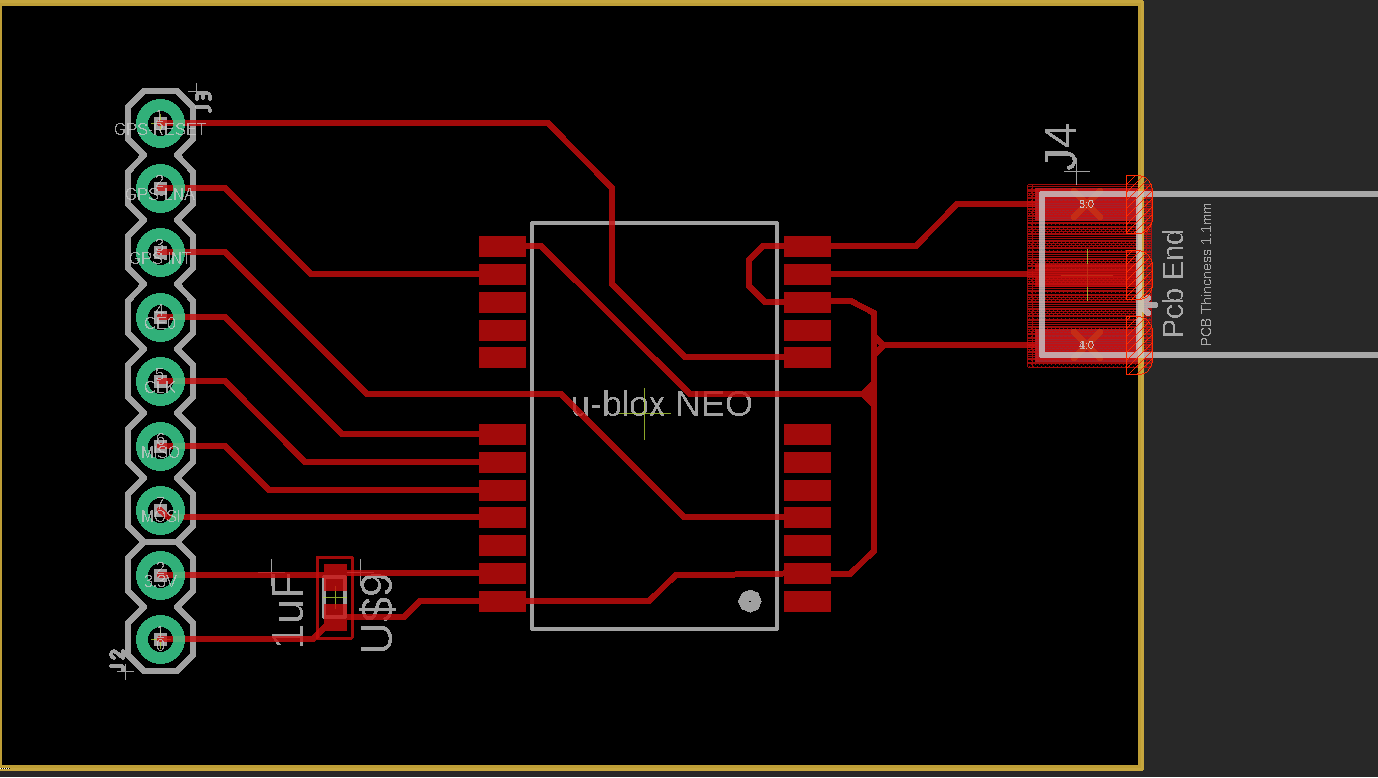
\includegraphics[width=.7\textwidth]{electrical/PCB_GPS.png}
           	\caption{PCB 1st iteration : GPS}
        \end{figure}
    \end{frame}
    
    
    \begin{frame}[c]{Electrical - Setup}
   		\begin{figure}[H]
            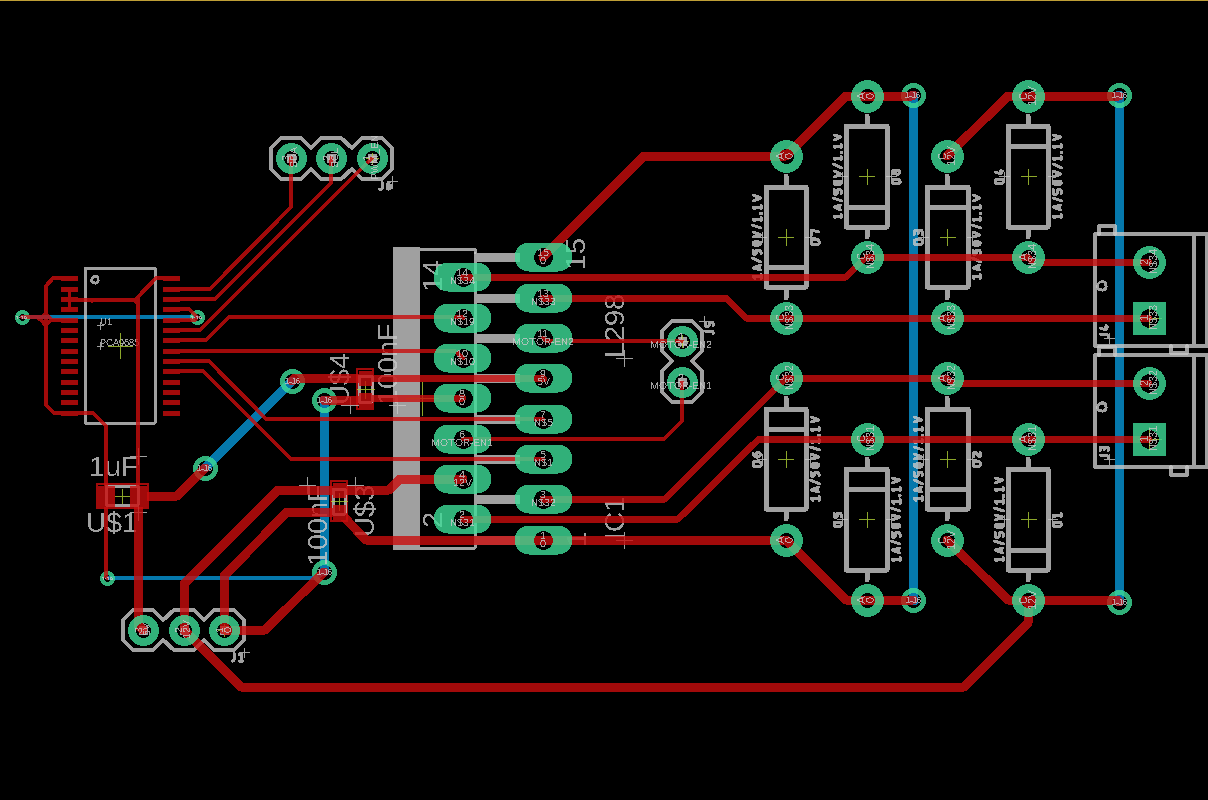
\includegraphics[width=.5\textwidth]{electrical/PCB_motorcontroll.png}
           	\caption{PCB 1st iteration : Motor Control}
        \end{figure}
    \end{frame}
    
    
    \begin{frame}[c]{Electrical - Setup}
   		\begin{figure}[H]
            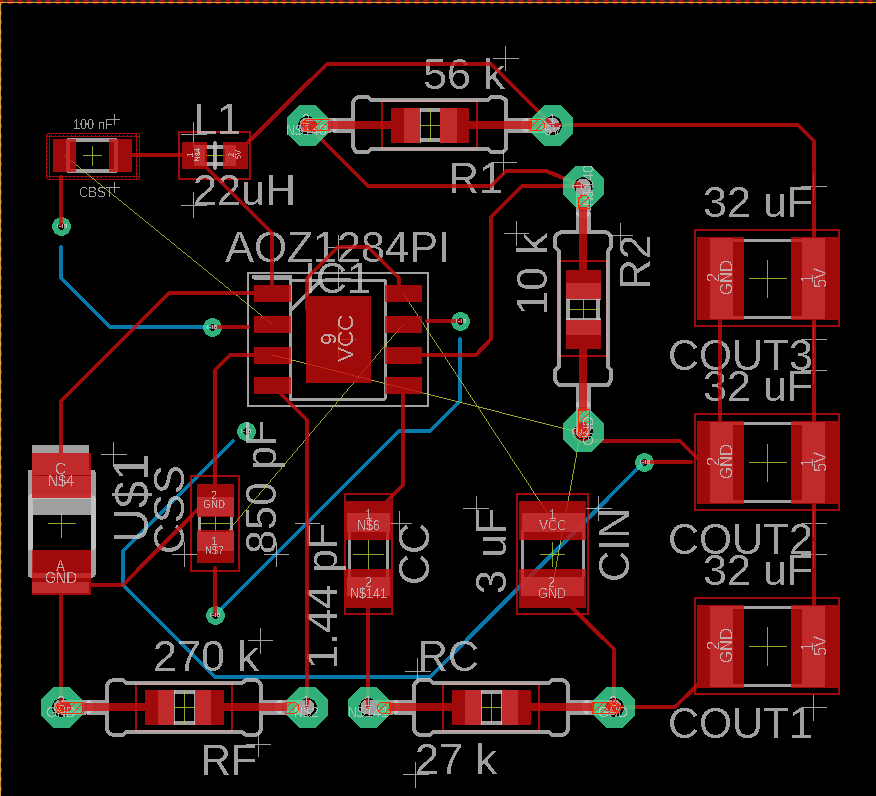
\includegraphics[width=.4\textwidth]{electrical/PCB_buck5v.png}
           	\caption{PCB 1st iteration : Buck Converter 5V}
        \end{figure}
    \end{frame}
    
    
    \begin{frame}[c]{Electrical - Setup}
   		\begin{figure}[H]
            \includegraphics[width=.4\textwidth]{electrical/IOextender.png}
           	\caption{PCB 1st iteration : IO extender}
        \end{figure}
    \end{frame}
    
\end{document}
